%\documentclass{sig-alternate-05-2015}
\documentclass[sigconf,review, anonymous]{acmart}
\acmConference[ESEC/FSE 2017]{11th Joint Meeting of the European Software Engineering Conference and the ACM SIGSOFT Symposium on the Foundations of Software Engineering}{4--8 September, 2017}{Paderborn, Germany}

\usepackage[utf8]{inputenc}
\usepackage[english]{babel}
\usepackage[T1]{fontenc}
\usepackage{graphicx}
\usepackage{graphics}
\usepackage{listings}  
\usepackage{array}
\newcolumntype{L}[1]{>{\raggedright\let\newline\\\arraybackslash\hspace{0pt}}m{#1}}
\newcolumntype{C}[1]{>{\centering\let\newline\\\arraybackslash\hspace{0pt}}m{#1}}
\newcolumntype{R}[1]{>{\raggedleft\let\newline\\\arraybackslash\hspace{0pt}}m{#1}}
\usepackage{multirow}
%\usepackage[table]{xcolor}
\usepackage{float}
\usepackage{array}
\usepackage{ragged2e}
\usepackage{cleveref}
\usepackage{subcaption}
\usepackage{tikz}

\newcolumntype{P}[1]{>{\RaggedRight\hspace{0pt}}p{#1}}

\lstset{language=Java,tabsize=2,basicstyle=\ttfamily\scriptsize} 

\newcommand{\squeezeup}{\vspace{-0.5mm}}

\usepackage{etoolbox}
\makeatletter
\patchcmd{\@makecaption}
{\scshape}
{}
{}
{}
\makeatother

\newcolumntype{"}{@{\hskip\tabcolsep\vrule width 1pt\hskip\tabcolsep}}

\lstdefinestyle{base}{
	language=C,
	emptylines=1,
	breaklines=true,
	basicstyle=\ttfamily\color{black},
	moredelim=**[is][\color{red}]{@}{@},
}

\newcommand\FIXME[1]{\textbf{FIXME: #1}}

\begin{document}

% Copyright
\setcopyright{acmcopyright}
%\setcopyright{acmlicensed}
%\setcopyright{rightsretained}
%\setcopyright{usgov}
%\setcopyright{usgovmixed}
%\setcopyright{cagov}
%\setcopyright{cagovmixed}


%% DOI
%\doi{10.475/123_4}

%% ISBN
%\isbn{123-4567-24-567/08/06}

%Conference
%\conferenceinfo{ESEC/FSE 2017}{September 4--8, 2017, Paderborn, Germany}

%\acmPrice{\$15.00}

%
% --- Author Metadata here ---
%\conferenceinfo{WOODSTOCK}{'97 El Paso, Texas USA}
%\CopyrightYear{2007} % Allows default copyright year (20XX) to be over-ridden - IF NEED BE.
%\crdata{0-12345-67-8/90/01}  % Allows default copyright data (0-89791-88-6/97/05) to be over-ridden - IF NEED BE.
% --- End of Author Metadata ---

\title{Are We Reusing Outdated and Licensed Code from Stack Overflow?}

%\numberofauthors{1}
\author{
	\alignauthor
	$^1$Chaiyong Ragkhitwetsagul, $^1$Matheus Paixao, $^1$Jens Krinke, $^2$Giuseppe Bianco \\
	\affaddr{$^1$University College London, London, UK}\\
	\affaddr{$^2$Università degli Studi del Molise, Campobasso, Italy}
}

\maketitle

\begin{abstract}
This paper provides a sample of a \LaTeX\ document which conforms,
somewhat loosely, to the formatting guidelines for
ACM SIG Proceedings. It is an {\em alternate} style which produces
a {\em tighter-looking} paper and was designed in response to
concerns expressed, by authors, over page-budgets.
It complements the document \textit{Author's (Alternate) Guide to
Preparing ACM SIG Proceedings Using \LaTeX$2_\epsilon$\ and Bib\TeX}.
This source file has been written with the intention of being
compiled under \LaTeX$2_\epsilon$\ and BibTeX.

The developers have tried to include every imaginable sort
of ``bells and whistles", such as a subtitle, footnotes on
title, subtitle and authors, as well as in the text, and
every optional component (e.g. Acknowledgments, Additional
Authors, Appendices), not to mention examples of
equations, theorems, tables and figures.

To make best use of this sample document, run it through \LaTeX\
and BibTeX, and compare this source code with the printed
output produced by the dvi file. A compiled PDF version
is available on the web page to help you with the
`look and feel'.
\end{abstract}

\section{Introduction}
%The popularity of the Internet encourages tremendous amount of source code being shared online. 
Stack Overflow is a popular online programming community with 6.3 million users. It allows programmers to ask questions and give answers to programming problems. The website has found to be useful for software development~\cite{Ponzanelli2013,Ponzanelli2014,Diamantopoulos2015,Keivanloo2014,Park2014, Stolee2014,Subramanian2013,Diamantopoulos2015,Treude2016} and also valuable for educational purposes~\cite{Nasehi2012}. On Stack Overflow, each conversation contains a question and answer(s).  The answers frequently contain at least one code snippet as a solution to the question asked. The code snippet is usually not written directly on Stack Overflow website but copied from another location. It can be copied and modified from the problematic code snippet in the question, copied from an answerer's own code, or borrowed from other locations including open source software (OSS) systems. The process of posting and answering questions on Stack Overflow, which involves copying and pasting source code, can be considered as code cloning. 

Code cloning is an activity of reusing source code by copying and pasting. It normally occurs in software development and account from 7\% to 23\% in typical software systems~\cite{Bellon2007}. The benefits and drawbacks of clones are still controversial. Several authors state that clones lead to bug propagations and software maintenance issues~\cite{Kamiya2002}, while some others have proofs that in some cases clones are not harmful than normal code or even beneficial~\cite{Saini2016,Kapser2006}. 

Code cloning can also have side effects of violating software licenses and software vulnerabilities. Carelessly cloning code from one project to another project with different license may cause software licensing violation~\cite{German2009}. This also happens within the context of online Q\&A website such as Stack Overflow. An et al.~\cite{An2017} showed that 1,279 cloned snippets between Android apps and Stack Overflow have potential of violating software licenses. Security is also among the main concerns when code is copied from online source. Stack Overflow helps developers to solve Android programming problems more quickly than other resources while, at the same time, gives less secure code than books and the official Android documentation~\cite{Acar2016}. Additionally, outdated and vulnerable third-party libraries from famous open source projects are cloned into in a large number of open source systems~\cite{Xia2014}.

% INTERESTING NEWS: http://www.theverge.com/tldr/2016/5/4/11593084/dont-get-busted-copying-code-from-stack-overflow

We call code snippets that are copied from software systems to online Q\&A websites (such as Stack Overflow), and vice versa as ``online code clones'' (sometimes only ``clones'' for brevity). There are four ways to create online code clones: (1) code is cloned from a software project to a Q\&A website as an example; (2) code is cloned from a Q\&A website to a software project to obtain a functionality, perform a particular task, or fixing a bug; (3) code is implicitly cloned from one software project to another by having a Q\&A website as a medium; and (4) code is cloned from an external source to both a software project and a Q\&A website. Online code clones can similarly lead to a problem of outdated code, bug propagation, licensing violation, and software vulnerability as classical code clones. Unfortunately, they are more difficult to locate and fix since the search space in online code corpora is larger and no longer confined in a local repository. 

In this study, we are interested in locating online code clones on Stack Overflow that are cloned from open source projects and study them on two aspects: obsoleteness and licensing issues. 

\begin{figure*}
	\begin{lstlisting}
          /* Code in Stack Overflow #22315734 */                         /* WritableComparator.java (2016-09-26) */
          public int compare (byte[] b1,int s1,int l1,                   public int compare(byte[] b1,int s1,int l1,
                              byte[] b2,int s2,int l2) {                                    byte[] b2,int s2,int l2) {
            try {                                                          try {
              buffer.reset(b1,s1,l1); /* parse key1 */                       buffer.reset(b1,s1,l1); /* parse key1 */
              key1.readFields(buffer);                                       key1.readFields(buffer);
              buffer.reset(b2,s2,l2); /* parse key2 */                       buffer.reset(b2,s2,l2); /* parse key2 */
              key2.readFields(buffer);                                       key2.readFields(buffer);
            } catch (IOException e) {                                        buffer.reset(null,0,0); /* clean up reference */
              throw new RuntimeException(e);                               } catch (IOException e) {
            }                                                                throw new RuntimeException(e);
            return compare(key1,key2); /* compare them */                  }
          }                                                                return compare(key1, key2); /* compare them */
	                                                                       }
	\end{lstlisting}
	\caption{A motivating example of the same code fragments, WritableComparator.java. The one on Stack Overflow post 22315734 is outdated when compared to its latest version in Hadoop code base}
	\label{fig:before-after}
\end{figure*}

A motivating example of outdated online code clones can be found in the a Stack Overflow post regarding how to implement {\small{\texttt{RawComparator}}} in \texttt{hadoop}\footnote{http://stackoverflow.com/questions/22262310}. In \Cref{fig:before-after}, the left hand side shows a code snippet embedded as a part of accepted answer to the question. The snippet shows how {\small{\texttt{hadoop}}} implements {\small{\texttt{compare}}} method in its {\small{\texttt{WritableComparator}}} class. The code snippet on the right hand side shows another version of the same {\small{\texttt{compare}}} method in {\small{\texttt{WritableComparator}}} class but it is extracted from the latest version of {\small{\texttt{hadoop}}}. We can obviously see that they are highly similar except one line, {\small{\verb|buffer.reset(null,0,0);|}}, is added in the latest version after {\small{\verb|key2.readFields(buffer);|}}. The added line is intended for cleaning up the reference in {\small{\verb|buffer|}} variable. While this change has already been introduced into {\small{\texttt{compare}}} method in the latest version of {\small{\texttt{hadoop}}}, the code example in Stack Overflow post is still unchanged. This example shows that there can be inconsistencies between online code clones and its original. The code snippet on Stack Overflow can be outdated.  %Since reusing source code from Stack Overflow is considered a common practice nowadays, the scale of online code cloning is more than intra or inter project clone in a local code bases. 
%This is an emerging and challenging problem. Since studies in this area are still limited, we aim to gain more insight of the problem in this study. %We are interested to gain more insights of online code clone in this study.

While a lot of research has focused on reusing code snippets ``from Stack Overflow'' (e.g.~\cite{Keivanloo2014,An2017,Yang2016}), less work has been conducted on finding the origins of code examples copied ``to Stack Overflow'' and effects of reusing them such as outdated code and software licensing violation.

To fill this gap, this paper makes the following  primary contributions:

\vspace{0.5ex}%
\noindent\textbf{1.~A manual study of online code clones:} 
We used two clone detection tools to discover 315,786,118 similar code snippet pairs and manually investigated 3,595 candidate clone pairs between Java code snippets obtained from Stack Overflow accepted answers and 111 Java open source projects.

\vspace{0.5ex}%
\noindent\textbf{2.~Addressing the problems of outdated and license-violating online clones on Stack Overflow:} Our study shows that there are at least 523 clones that have been obviously copied from open source projects or external online sources to Stack Overflow as code examples which potentially violate their software licenses. Importantly, 53 out of the 96 online code clones on Stack Overflow are outdated and questionable for being reused.

\vspace{0.5ex}%
\noindent\textbf{3.~Online code clone oracle:} The 3,632 manually investigated and validated online clone pairs are available for download on the study website\footnote{https://to.be.disclosed.after.review} and can be used as a clone oracle.

\section{Empirical Study}
We performed an empirical study of online code clones between Stack Overflow and 109 Java open source projects to answer the following research questions: \\ 
\textbf{RQ1 (online code clones):} \textit{To what extent  source code is cloned between Stack Overflow and open source projects?} We quantitatively measured the number of online code clones between Stack Overflow and open source projects to understand the scale of the problem. \newline
%\textbf{RQ2 (flow of online code clones):} \textit{what are the directions that source code is cloned?} If clones between the two locations exist, we would like to observe in which direction the code has been copied. Is it mostly from Stack Overflow to open source projects, or the other way around, or equally both? \newline
\textbf{RQ2 (Patterns of online code clones):} \textit{Why do online code clones occur?} We categorised online clones into seven categories according to our online code cloning pattern scheme. This gave us more insights to why online code clones are created. %so we can differentiate and understand the motivation of cloning. 
%Clones can be copied from open source projects to Stack Overflow as examples, or vice versa. Furthermore, they can be cloned from a third-party location or clones containing boiler-plate code, and code stubs generated by IDE. \newline
\newline
\textbf{RQ3 (Outdated online code clones):} \textit{Are online code clones up-to-date compared to their counterparts in the original projects?} We were interested in the correctness of Stack Overflow code examples since millions of users are potentially reusing them.  %Is there observable problems caused by clones between Stack Overflow and open source projects? 
%We are interested to investigate the problem of outdated code and software licensing conflicts caused by online code clones.

\textbf{RQ4 (Software licensing violation):} \textit{Do licensing conflicts occur between Stack Overflow clones and their originals?} We investigated whether online code clones can be legally harmful to software reusing them.

\begin{figure}
	\centering
	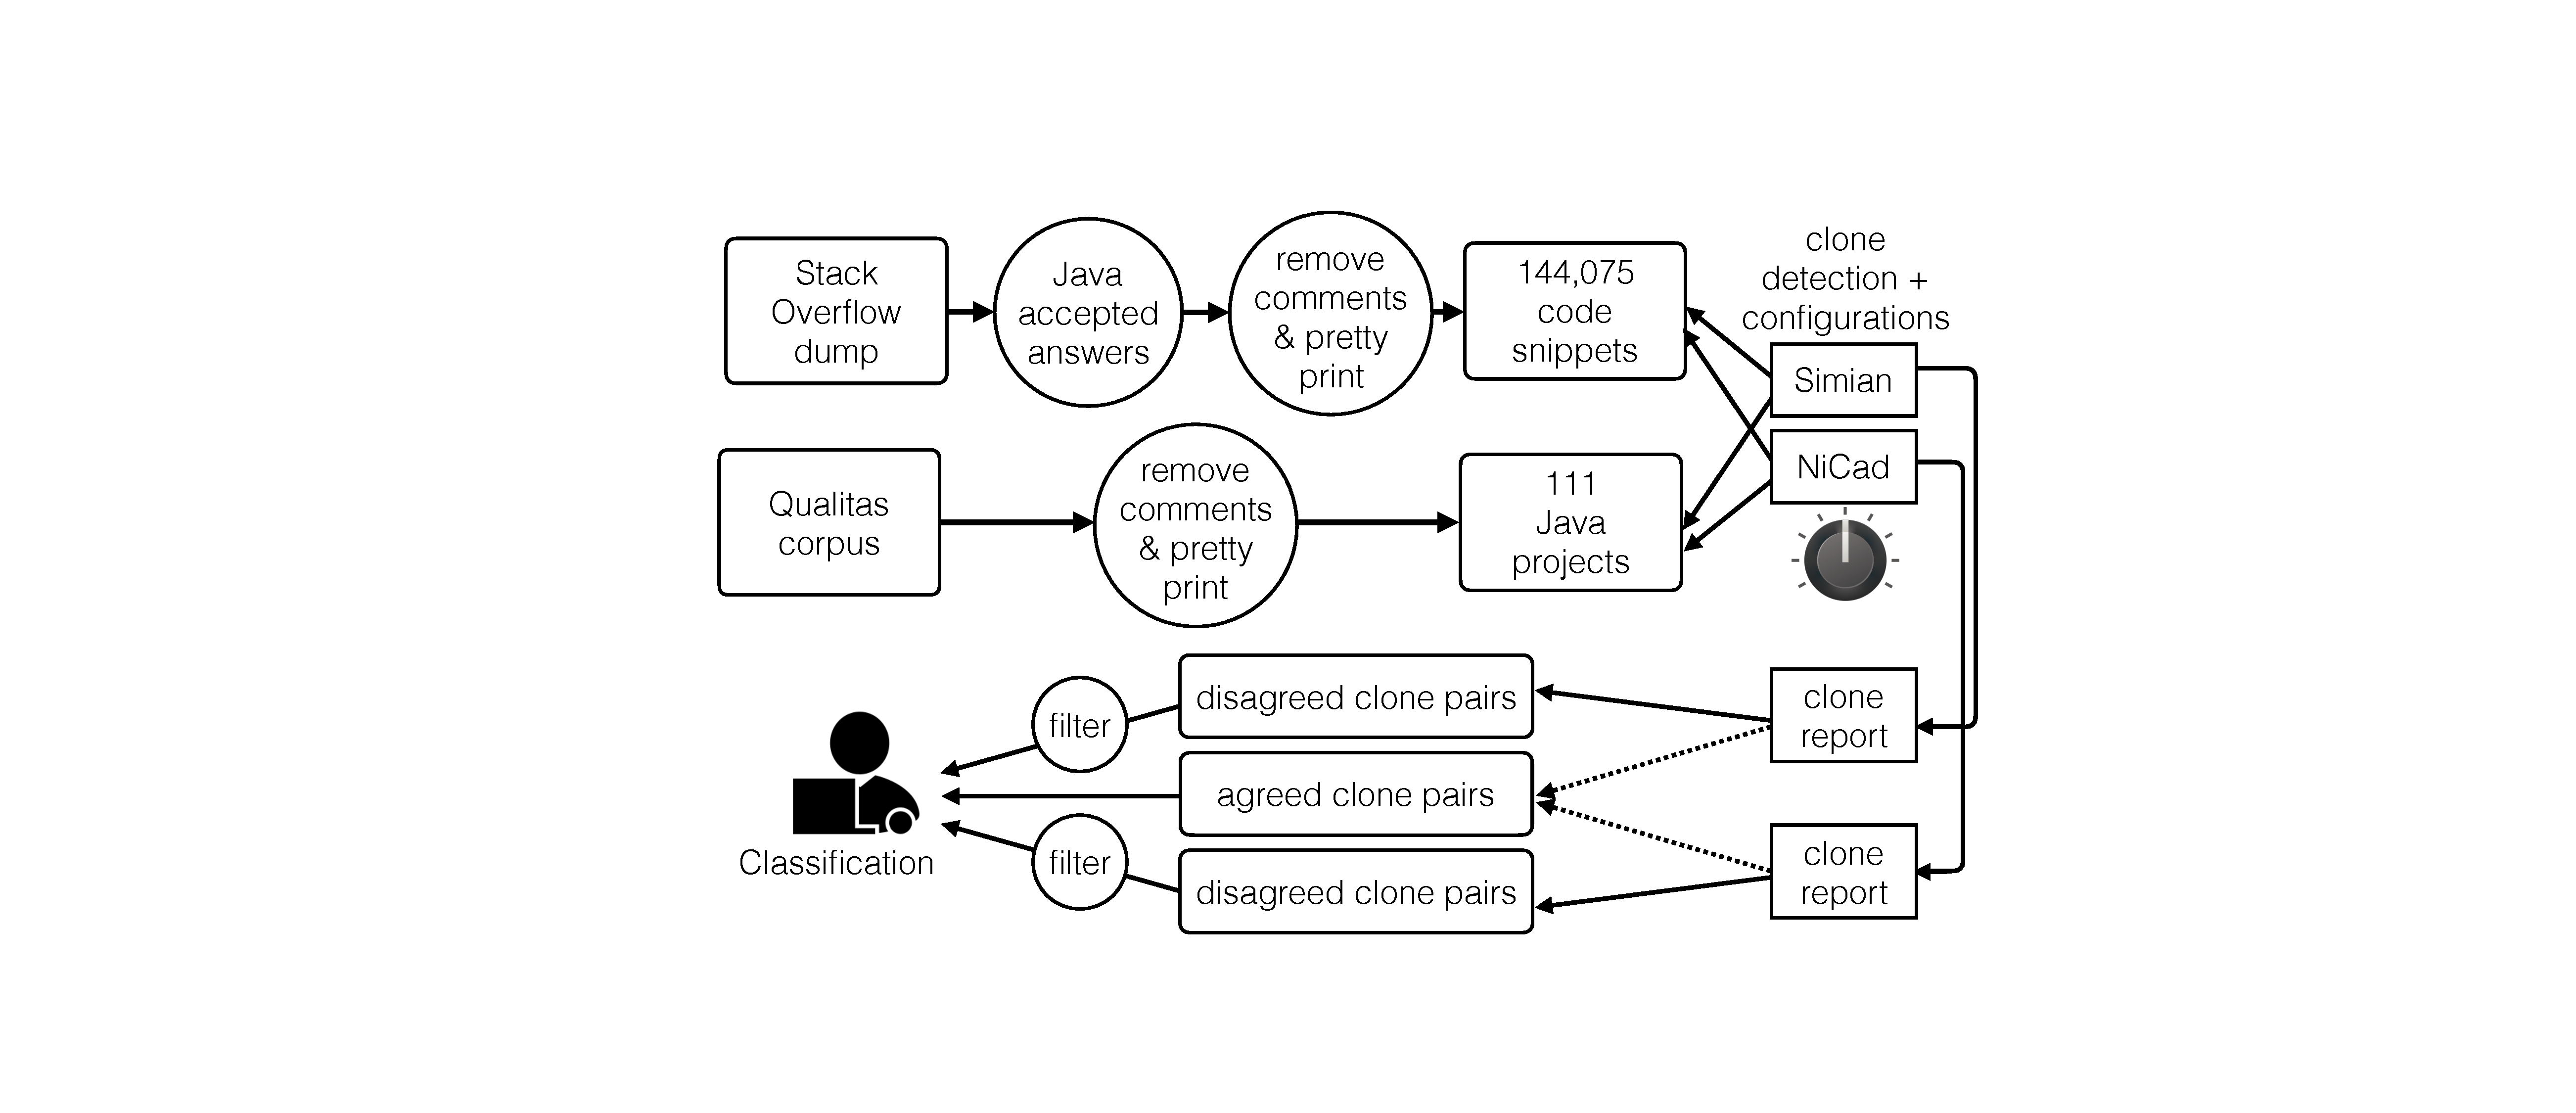
\includegraphics[width=0.8\linewidth]{exp_framework_new}
	\caption{Experimental framework}
	\label{fig:exp_framework}
\end{figure}

\subsection{Experimental Framework}
To answer the four research questions, we followed the experimental framework depicted in \Cref{fig:exp_framework}. We processed two datasets, Stack Overflow and 111 open source projects from Qualitas corpus. Java code snippets were extracted from Stack Overflow posts using regular expressions. We prepared Java code in both datasets by removing comments and pretty-printing to increase accuracy of clone detection. Then, we deployed two clone detection tools, Simian~\cite{simian} and NiCad~\cite{Roy2008,Cordy}, to locate clones between the two datasets. Due to scalability of Simian and NiCad, we partitioned the input and run the tools multiple times. Each run was composed of the whole Stack Overflow data and single Qualitas project. We repeated the process until we cover 111 projects. 

We then converted the clone reports to General Clone Format (GCF)~\cite{Wang2013} and combined the 111 reports into a single GCF file. GCF provides a common format for clones which enabled us to reuse the same scripts to analyse clone reports from both Simian and NiCad. Moreover, using GCF, other additional clone detectors could be adopted, if needed, without any changes in the analysis. Simian did not provide an option to detect inter clones between two locations. Hence the Simian GCF clone report was pruned to contain only inter clone pairs between Stack Overflow and Qualitas projects. In this step, all intra clone pairs within either Stack Overflow or Qualitas were removed. NiCad provided an option to detect inter clones so no pruning is needed. We did not have an oracle of clones between the two data sets so we rely on a manual investigation to validate the reported clone candidates. However, the large amount of clone pairs hindered us from looking at all of them. Random sampling of clones could be done but may return mostly non-meaningful clones. Instead, we selected clone pair candidates by relying on agreement of clone detectors. If a clone pair was similarly reported by multiple tools, we had a higher confidence that it was a real clone pair. To achieve this, clone pairs from the two clone detectors were pair-wise matched to find agreements using Bellon's clone overlapping criteria~\cite{Bellon2007}. This step generated \textbf{agreed clone pairs}. They were pairs with high confidence to be true clones since they obtained agreement from both tools. Then, pairs reported by Simian and NiCad that did not find agreement were \textbf{disagreed clone pairs}. The disagreed clone pairs were clones with less confidence than the agreed ones. Finally, agreed and disagreed clone pairs had been looked at manually by the first and the third author.

In the manual inspection process, we classified clones into seven categories according to information observed from code comments and natural text in Stack Overflow answer. This process took approximately a months until we successfully investigated 3,450 clone pairs. Clone pairs that were classified as false clones, boiler-plate code, or IDE-generated were not very interesting and were ignore in the analysis of outdated code and licensing violation. 
We compared licensing information of 523 remaining clone pairs for possibility of software licensing violations. Moreover, we looked forward through history of each clone from its git repository. With this method, we discovered \textbf{outdated code}, code that changes are made to them after it had been copied to Stack Overflow. %hence resulting in outdated clones on Stack Overflow.

\subsection{Experimental Setup}

\subsubsection{Datasets}

\textbf{Stack Overflow}: we extracted Java code snippets from a snapshot of Stack Overflow dump \footnote{https://archive.org/details/stackexchange} in January 2016. The archived dump has a size of 9 gigabytes. The data dump was in XML format containing information of \textbf{Posts} (questions and answers) and supporting data such as user accounts and timestamps of the posts. We were interested in code snippets embedded in posts which were located between {\small\texttt{<code></code>}} tags. A Stack Overflow thread contains a post of question and several posts of answers. Every answer has voting score from its users. An answer can also be marked as \textbf{accepted answer} by the questioner if the solution fixes his/her problem. We collected Java code snippets using two criteria. First, we were only interested in code snippets with at least six lines. Snippets which were smaller than six lines were usually spurious clones~\cite{Bellon2007}. Second, we only focused on code snippets in accepted answers. We chose the snippets in accept answers because they actually solved the problems in the questions and had a check mark sign on them to notify other users. Moreover, they were always displayed just below the questions which made them attractive to be reused than other answers. Each snippet was extracted from the dump using regular expressions and saved to a file using its post ID as the file's name. If an accepted answer had more than one code snippet, we appended an indexing number, starting from zero, after the post ID (e.g. 45051109\_0, and 45051109\_1.). Lastly, we added {\small\texttt{.java}} extension to the file's names so that clone detectors could recognise them. We finally obtained 144,075 Java code snippets which contain 2,347,269 lines of Java source code excluding comments and blank lines\footnote{Measured by cloc: https://github.com/AlDanial/cloc}.

\textbf{Open source systems}: we selected an established corpus for an empirical software engineering study called \textbf{Qualitas}~\cite{QualitasCorpus} for this study. It is a curated Java corpus that has been used in several software engineering studies~\cite{Taube-Schock2011,Beckman2011,Vasilescu2011,Omar2012}. The projects in the corpus represent various domains of software systems ranging from programming language to 3D and visualisation~\cite{QualitasCorpus}. We selected the 20130901r release of Qualitas corpus containing 112 Java open source projects. This release contains projects with releases no later than 1st September 2013. We chose a snapshot late back in 2013 since we are interested in online code clones in the direction from open source projects to Stack Overflow. The 20130901r snapshot provides Java code that is at least 3 years old from the time of the experiment (January to December 2016). The time difference is sufficiently long for a number of code snippets to be copied onto Stack Overflow. Out of 112 Qualitas projects, there is one project, \texttt{jre}, that does not contain Java source code due to its licensing limitation~\cite{QualitasCorpus} so it is removed from the study. This resulted in total of 111 projects analysed in the study. As shown in \Cref{tab:datasets}, the 111 Qualitas project have 160,937 Java files containing 19,086,883 lines of code. %Details of the 109 Qualitas projects and their licenses are listed in Table \ref{t:new_and_old}.

\begin{table}
	\centering
	\caption{Stack Overflow and Qualitas datasets}
	\label{tab:datasets}
	\small
	\begin{tabular}{l|r|r}
		\hline 
		Dataset & No. of files & SLOC \\
		\hline
		Stack Overflow & 144,075 & 2,347,269 \\ 
		\hline 
		Qualitas &  160,937 & 19,086,883 \\ 
		\hline 
	\end{tabular} 
\end{table}

\subsubsection{Clone Detectors}
There is a number of restrictions in terms of choosing clone detection tools for this study. First, they have to support Java. Second, due to nature of code snippets posted on Stack Overflow, some of them are not complete Java classes or methods. Hence, the tool must be flexible enough to process code snippets that are neither a complete block nor compilable. Third, since the amount of code that have to be processed are in a scale of millions line of code (as shown in \Cref{tab:datasets}), a clone detector must be scalable enough to successfully complete the execution and report clones in a reasonable amount of time. We have tried running 5 state-of-the-art clone detectors including Simian~\cite{simian}, NiCad~\cite{Cordy,Roy2008}, CCFinder~\cite{Kamiya2002}, iClones~\cite{Gode2009}, and DECKARD~\cite{Jiang2007a} against Stack Overflow and Qualitas datasets. CCFinder, iClones, and DECKARD failed to report clones between 144,075 Stack Overflow code snippets and 111 Qualitas projects. All of them reported execution errors after running for couple of hours. Thus, we removed them from the study. Simian and NiCad completed the detection with success. We found that both of them are also flexible enough to handle code with incomplete methods or classes. %So, we decided to use both of them.

\textbf{Simian} is a text-based clone detector which locate clones at line-level granularity and has been used extensively in several clone studies~\cite{Ragkhitwetsagul2016, Wang2013, Mondal2011, Cheung2015, Krinke2010}. It is a command-line tool which enables us to automate the detection. Furthermore, it offers normalisation of variable names and literals (strings, and numbers) which enable Simian to detect literal clones (type-1) and parameterised clones (type-2). \textbf{NiCad} is also a text-based clone detector which detects clones at either method- or block-level granularity. It can detect clones of type-1, 2 up to type-3 (clones with added/removed/relocated/changed statements) and is also used in several empirical clone studies~\cite{Roy2008, Ragkhitwetsagul2016, Svajlenko2014, Wang2013, Mondal2011, Sajnani2016}. It utilises TXL~\cite{Cordy2006} for parsing and pretty-printing source code. It also provide code normalisation by variable renaming and abstraction. We use a variant of NiCad called \textit{nicadcross}. It offers the same functionalities as the original NiCad but is specialised for detecting code clones between two systems. NiCad is also a command-line tool which makes it suitable for automation.

\subsubsection{Prioritise Clone Candidates Using Agreement}
A number of clones detected in large-scale datasets can be huge. In our study, there are totally 266,837,480 clone pairs reported. It is almost infeasible for human to manually validate them all. One can do a random sampling of clones. However, due to a very high number of false positives, they may end up looking at most of the false clones. Therefore, we adopted an idea of \textbf{clone agreement} which has been used in clone research studies~\cite{Wang2013,Funaro2010,cr2016ssbse} in a situation that clone oracle is missing or impossible to establish. Clone pairs agreed by multiple clone detection tools have higher confident to be real clones~\cite{cr2016ssbse}. By using this agreement-based approach, we could reduce the number of clone candidates for manual investigation by paying more attention to the ones agreed by multiple tools. To find an agreement between two clone pairs report by two different tools, we used clone pair matching metric proposed by Bellon et al.~\cite{Bellon2007}. Two clone pairs which have large enough overlapping clone lines can be categorised as either a good-match or an ok-match pair (denoted as \textit{good} and \textit{ok} respectively) with a confident value between 0 and 1. A \textit{good} clone pair has stronger agreement than an \textit{ok} pair. We follow the following definitions of good- and ok-match introduced in the original paper.

\vspace{0.5ex}
Given that a clone pair \textit{CP} is formed by two clone fragments \textit{CF$_1$} and \textit{CF$_2$} with a pre-defined similarity threshold \textit{t}, i.e.~\textit{CP} = (\textit{CF$_1$}, \textit{CF$_2$}, \textit{t}), we can define \textit{overlap} and \textit{contained} value of two clone pairs as 
%\squeezeup
\begin{multline}
	overlap(\textrm{\textit{CP}}_1, \textrm{\textit{CP}}_2) = \frac{|lines(\textrm{\textit{CF}}_1) \cap lines(\textrm{\textit{CF}}_2)|}{|lines(\textrm{\textit{CF}}_1) \cup lines(\textrm{\textit{CF}}_2)|} 
\end{multline}
%\squeezeup
\begin{multline}
	contained(\textrm{\textit{CP}}_1, \textrm{\textit{CP}}_2) = \frac{|lines(\textrm{\textit{CF}}_1) \cap lines(\textrm{\textit{CF}}_2)|}{|lines(\textrm{\textit{CF}}_1)|}. 
\end{multline}

\noindent\textit{good-value} of two clone pairs is then defined as
%\squeezeup
\begin{align*}
	good(\textrm{\textit{CP}}_1, \textrm{\textit{CP}}_2) = min(overlap(\textrm{\textit{CP}}_1.\textrm{\textit{CF}}_1,\textrm{\textit{CP}}_2.\textrm{\textit{CF}}_1), \\ overlap(\textrm{\textit{CP}}_1.\textrm{\textit{CF}}_2,\textrm{\textit{CP}}_2.\textrm{\textit{CF}}_2)).
\end{align*}

\noindent\textit{ok-value} is defined as
%\squeezeup
\begin{align*}
	ok(\textrm{\textit{CP}}_1,\textrm{\textit{CP}}_2) = min(max(contained(\textrm{\textit{CP}}_1.\textrm{\textit{CF}}_1,\textrm{\textit{CP}}_2.\textrm{\textit{CF}}_1), \\ contained(\textrm{\textit{CP}}_2.\textrm{\textit{CF}}_1,\textrm{\textit{CP}}_1.\textrm{\textit{CF}}_1)),
	\\ max(contained(\textrm{\textit{CP}}_1.\textrm{\textit{CF}}_2,\textrm{\textit{CP}}_2.\textrm{\textit{CF}}_2), \\contained(\textrm{\textit{CP}}_2.\textrm{\textit{CF}}_2,\textrm{\textit{CP}}_1.\textrm{\textit{CF}}_2))).
\end{align*}

Two clone pairs $\textrm{\textit{CP}}_1$ and $\textrm{\textit{CP}}_2$ are called a \textit{\textit{good}(p)} iff, for $p \in [0,1]$ holds 
%\squeezeup
\begin{equation}
good(\textrm{\textit{CP}}_1,\textrm{\textit{CP}}_2) \geq p.
\end{equation}

Similarly for an \textit{ok-match(p)} pair
%\squeezeup
\begin{equation}
ok(\textrm{\textit{CP}}_1,\textrm{\textit{CP}}_2) \geq p.
\end{equation}

Using this good and ok-match criteria with a predefined threshold \textit{p}, we can prune the 266-million candidate clone pairs for manual investigation. \textit{good} pairs are the ones with the highest confident and ranked the first to be looked at, followed by \textit{ok} pairs, and followed by clone pairs without agreement.

\subsection{Clone Detector's Parameter Tuning}
We were aware of effects of configurations to clone detection results and the importance of searching for optimised configurations in empirical clone studies~\cite{Wang2014,cr2016ssbse,Ragkhitwetsagul2016,Svajlenko2014}. However, considering the massive size of the two datasets and search space of at least 15 Simian's and 5 NiCad's parameters, we were hindered from searching for the best configurations of the tools. Thus, we decided to configure Simian and NiCad using two established configurations: 1) the tools' default configurations chosen by the tools' creators (denoted as \textit{D}), and 2) the discovered configurations for Bellon's Java projects from \textit{EvaClone}, a study of optimising clone detectors' configurations based on clone agreement, by Wang et al.~\cite{Wang2013} (denoted by \textit{E}). The details of the two configurations are described in \Cref{t:param_tuning}. Having two clone detectors, Simian (denoted as \textit{S}) and NiCad (denoted as \textit{N}), with two chosen configurations each, we looked for Bellon's good and ok-match in four possible pair-wise combinations: $S_{D}N_{D}$, $S_{D}N_{E}$, $S_{E}N_{D}$, and $S_{E}N_{E}$.

\begin{table}
	\centering
	\caption{Configurations of Simian and NiCad}
	\label{t:param_tuning}
%	\resizebox{\columnwidth}{!}{%
	\small
	\begin{tabular}{l|p{7cm}}
		\hline 
		Tool & Parameters \\
		\hline
		$S_D$ &  threshold=6, ignoreStringCase, \newline ignoreCharacterCase, ignoreModifiers \\ 
		\hline
		$S_E$ & threshold=5, ignoreIdentifiers, \newline ignoreIdentifierCase, ignoreStrings, \newline ignoreCharacters, ignoreSubtypeNames, \newline balanceSquareBrackets  \\ 
		\hline 
		$N_D$ & Blocks, MinLine=10, MaxLine=1000, UPI=0.30 \\
		\hline
		$N_E$ & Blocks, MinLine=5, MaxLine=604, UPI=0.20, \newline blind renaming, literal abstraction \\ 
		\hline 
	\end{tabular} %
%}
\end{table}

\section{Results and Discussion}

We followed the experimental framework and detected clones between Stack Overflow and Qualitas corpus using the two selected clone detectors. To answer RQ1, we computed statistics of clone discovered by the tools. To answer RQ2, we manually investigated online clone pair candidates and categorised them using our patterns of online code cloning. The patterns were derived from Kapser et al.~\cite{Kapser2003} augmented by common patterns found in our data set. For RQ3, we looked at the true positive clone pairs and check if they are still up-to-date. Similarly, for RQ4, we also looked at the license of each clone and observed a possibility of licensing violation.

\subsection{RQ1: Online Code Clones} 

\begin{table}
	\centering
	\caption{Statistics of clones found between Stack Overflow and Qualitas projects using Simian (\textit{S}) and NiCad (\textit{N}) with default (\textit{D}) and EvaClone (\textit{E}) configurations \FIXME{boxplots here?}}
	\label{tab:raw_stats}
	\small
%	\resizebox{\columnwidth}{!}}}$ & 29\% & 28\% & 25\% & 21\% \\
			\hline
		\end{tabular} %
%	}
\end{table}

The clone statistics obtained from running Simian and NiCad with \textit{D} and \textit{E} configurations are presented in \Cref{tab:raw_stats}. From \Cref{tab:raw_stats}, Simian clones cover approximately 1\% of the 144,075 Stack Overflow snippets, 1,086 reported by $S_D$ and 1,531 from $S_E$ respectively. $N_D$ reports clones in 1,392 Stack Overflow code snippets, while $N_E$ reports clones in a larger number of 12,886 snippets  mainly due to its relaxed configurations. In terms of number of clone pairs, $S_E$ and $N_E$ report a large number of clone pairs of 63,635,844 and 251,449,849 respectively. This is expected since EvaClone configurations prefer recall so it tends to remote more clones~\cite{Wang2013}. The average clone size of $S_D$ is 7.72 lines which is bigger than its $S_E$ counterpart of 4.79. Similarly, $N_D$ has an average clone size of 9.84 lines which is bigger than 5.33 reported by $N_E$. We can see from the statistics that EvaClone tunes the tools in the way that they report smaller clones. The average percentage of Stack Overflow code snippets that are cloned according to $S_D$, $S_E$, $N_D$, and $N_E$ is 29\%, 28\%, 25\%, and 21\% accordingly. A quick manual check of Simian's clone report revealed that there were problematic 11 snippets. These 11 snippets triggered Simian to generate large clone clusters containing a huge number of false clones from array initialisation. Hence, their clones were removed from further analyses. 

As displayed in \Cref{tab:online_clone_pairs}, after we applying clone agreement filtering using Bellon's criteria, the number of \textit{good} agreed clone pairs is 2,308 while \textit{ok} is 11,749. The number of disagreed clone pairs ($S_D$, $N_D$) after filtering is 17,801 and 181 for Simian and NiCad respectively. The total number of clone candidates is 32,039 pairs. The details are as follows.

\begin{table}
	\centering
	\caption{The number of online clone pair condidates (mutually exclusive) before and after filtering.}
	\label{tab:online_clone_pairs}
	\small
%	\resizebox{\columnwidth}{!}{%
	\begin{tabular}{l|r|c|c|c|c|r}
		\hline
		\multirow{2}{*}{Set} & \multicolumn{1}{c|}{Before} & \multicolumn{4}{c|}{Filters*} & \multirow{2}{*}{Cand.} \\ \cline{3-6}
		& \multicolumn{1}{c|}{Filters} & \textit{L} & \textit{S} & \textit{R} & \textit{G} & \\
		\hline 
		\multirow{1}{*}{\textit{good}} & 2,308 & & & & & 2,308 \\
		\multirow{1}{*}{\textit{ok}} & 11,749 & & & & & 11,749 \\
		%\multirow{1}{*}{\textit{agreed clone pairs}}      & 29,099 \\
		\multirow{1}{*}{$S_D$} & 67,570 & \checkmark & & \checkmark & \checkmark & 17,801 \\
		\multirow{1}{*}{$N_D$} & 229,176 & & \checkmark & \checkmark & \checkmark & 88 \\ 
		%\multirow{1}{*}{\textit{disagreed clone pairs}}    & 1,039 \\
		\hline
		Total  & 310,803 & & & & & 31,946 \\ 
		\hline
		\multicolumn{7}{l}{Filters*: \textit{L}=$Line \geq 10$, \textit{S}=$Sim \geq 85\%$,} \\
		\multicolumn{7}{l}{\textit{R}=regular expressions, and \textit{G}=\textit{good}/\textit{ok} pairs.} \\
	\end{tabular} %
%}
\end{table}

\begin{table}
	\centering
	\caption{The online clone classification results}
	\label{tab:online_clone_classification_results}
	\small
	%	\resizebox{\columnwidth}{!}{%
	\begin{tabular}{l|r|r|r|r}
		\hline
		\multirow{2}{*}{Set} & \multirow{2}{*}{Candidates} & \multicolumn{2}{c|}{Classification} & \multirow{2}{*}{TP} \\ \cline{3-4}
		& & Auto & Manual & \\
		\hline 
		\multirow{1}{*}{\textit{good}} & 2,308 & 10 & 2,298 & 18 \\
		\multirow{1}{*}{\textit{ok}} & 11,749 & 11,494 & 255 & 75 \\
		%\multirow{1}{*}{\textit{agreed clone pairs}}      & 29,099 \\
		\multirow{1}{*}{$S_D$} & 17,801 & 16,800 & 1,001 & 525 \\
		\multirow{1}{*}{$N_D$} & 88 & 10 & 78 & 50 \\ 
		%\multirow{1}{*}{\textit{disagreed clone pairs}}    & 1,039 \\
		\hline
		Total  & 31,946 & 28,314 & 3,632 & 668 \\ 
		\hline
	\end{tabular} %
	%}
\end{table}

\subsubsection{Agreed clone pairs}

Agreed clone pairs are clone pairs that pass Bellon's good- or ok-match criteria and selected for manual investigation. Similar to the original study, we select a threshold \textit{p} of 0.7 for both \textit{good} and \textit{ok} pairs~\cite{Bellon2007}. %The number of projects processed by the clone detection tools are listed in \Cref{tab:projects_missing}. 
We encountered NiCad failures with a few Qualitas projects.~$N_D$ could not detect clones in \texttt{hibernate} due to clustering errors. $N_E$ generated renaming errors for 5 projects including \texttt{vuze}, \texttt{hibernate}, \texttt{myfaces}, \texttt{netbeans}, and \texttt{spring}. We had contacted the creator of NiCad regarding the issues. They identified them as problems of long file paths and TXL grammars which will be fixed in the next NiCad releases. As a result, we did not have NiCad clones from these projects in the agreed clone pairs. Simian clones of the same projects also disappeared from the agreed clone pairs since they could not find matches.

\begin{table}
	\centering
	\caption{Distribution of the agreed clone pairs}
	\label{t_agreed_good_clone_pairs}
	\small
%	\resizebox{\columnwidth}{!}{%
	\begin{tabular}{l|r|r|r|r|r|r}
		\hline
		Set & $S_DN_D$ & $S_DN_E$ & $S_EN_D$ & $S_EN_E$ & Total & Unique \\
		\hline
		\textit{good} & 18 & 26 & 10 & 2,267 & 2,321 & 2,308 \\
		\textit{ok} & 11,467 & 993 & 79 & 20,021 & 32,560 & 31,729  \\
		\hline
	\end{tabular} %
%}
\end{table}

\begin{figure}
	\centering
	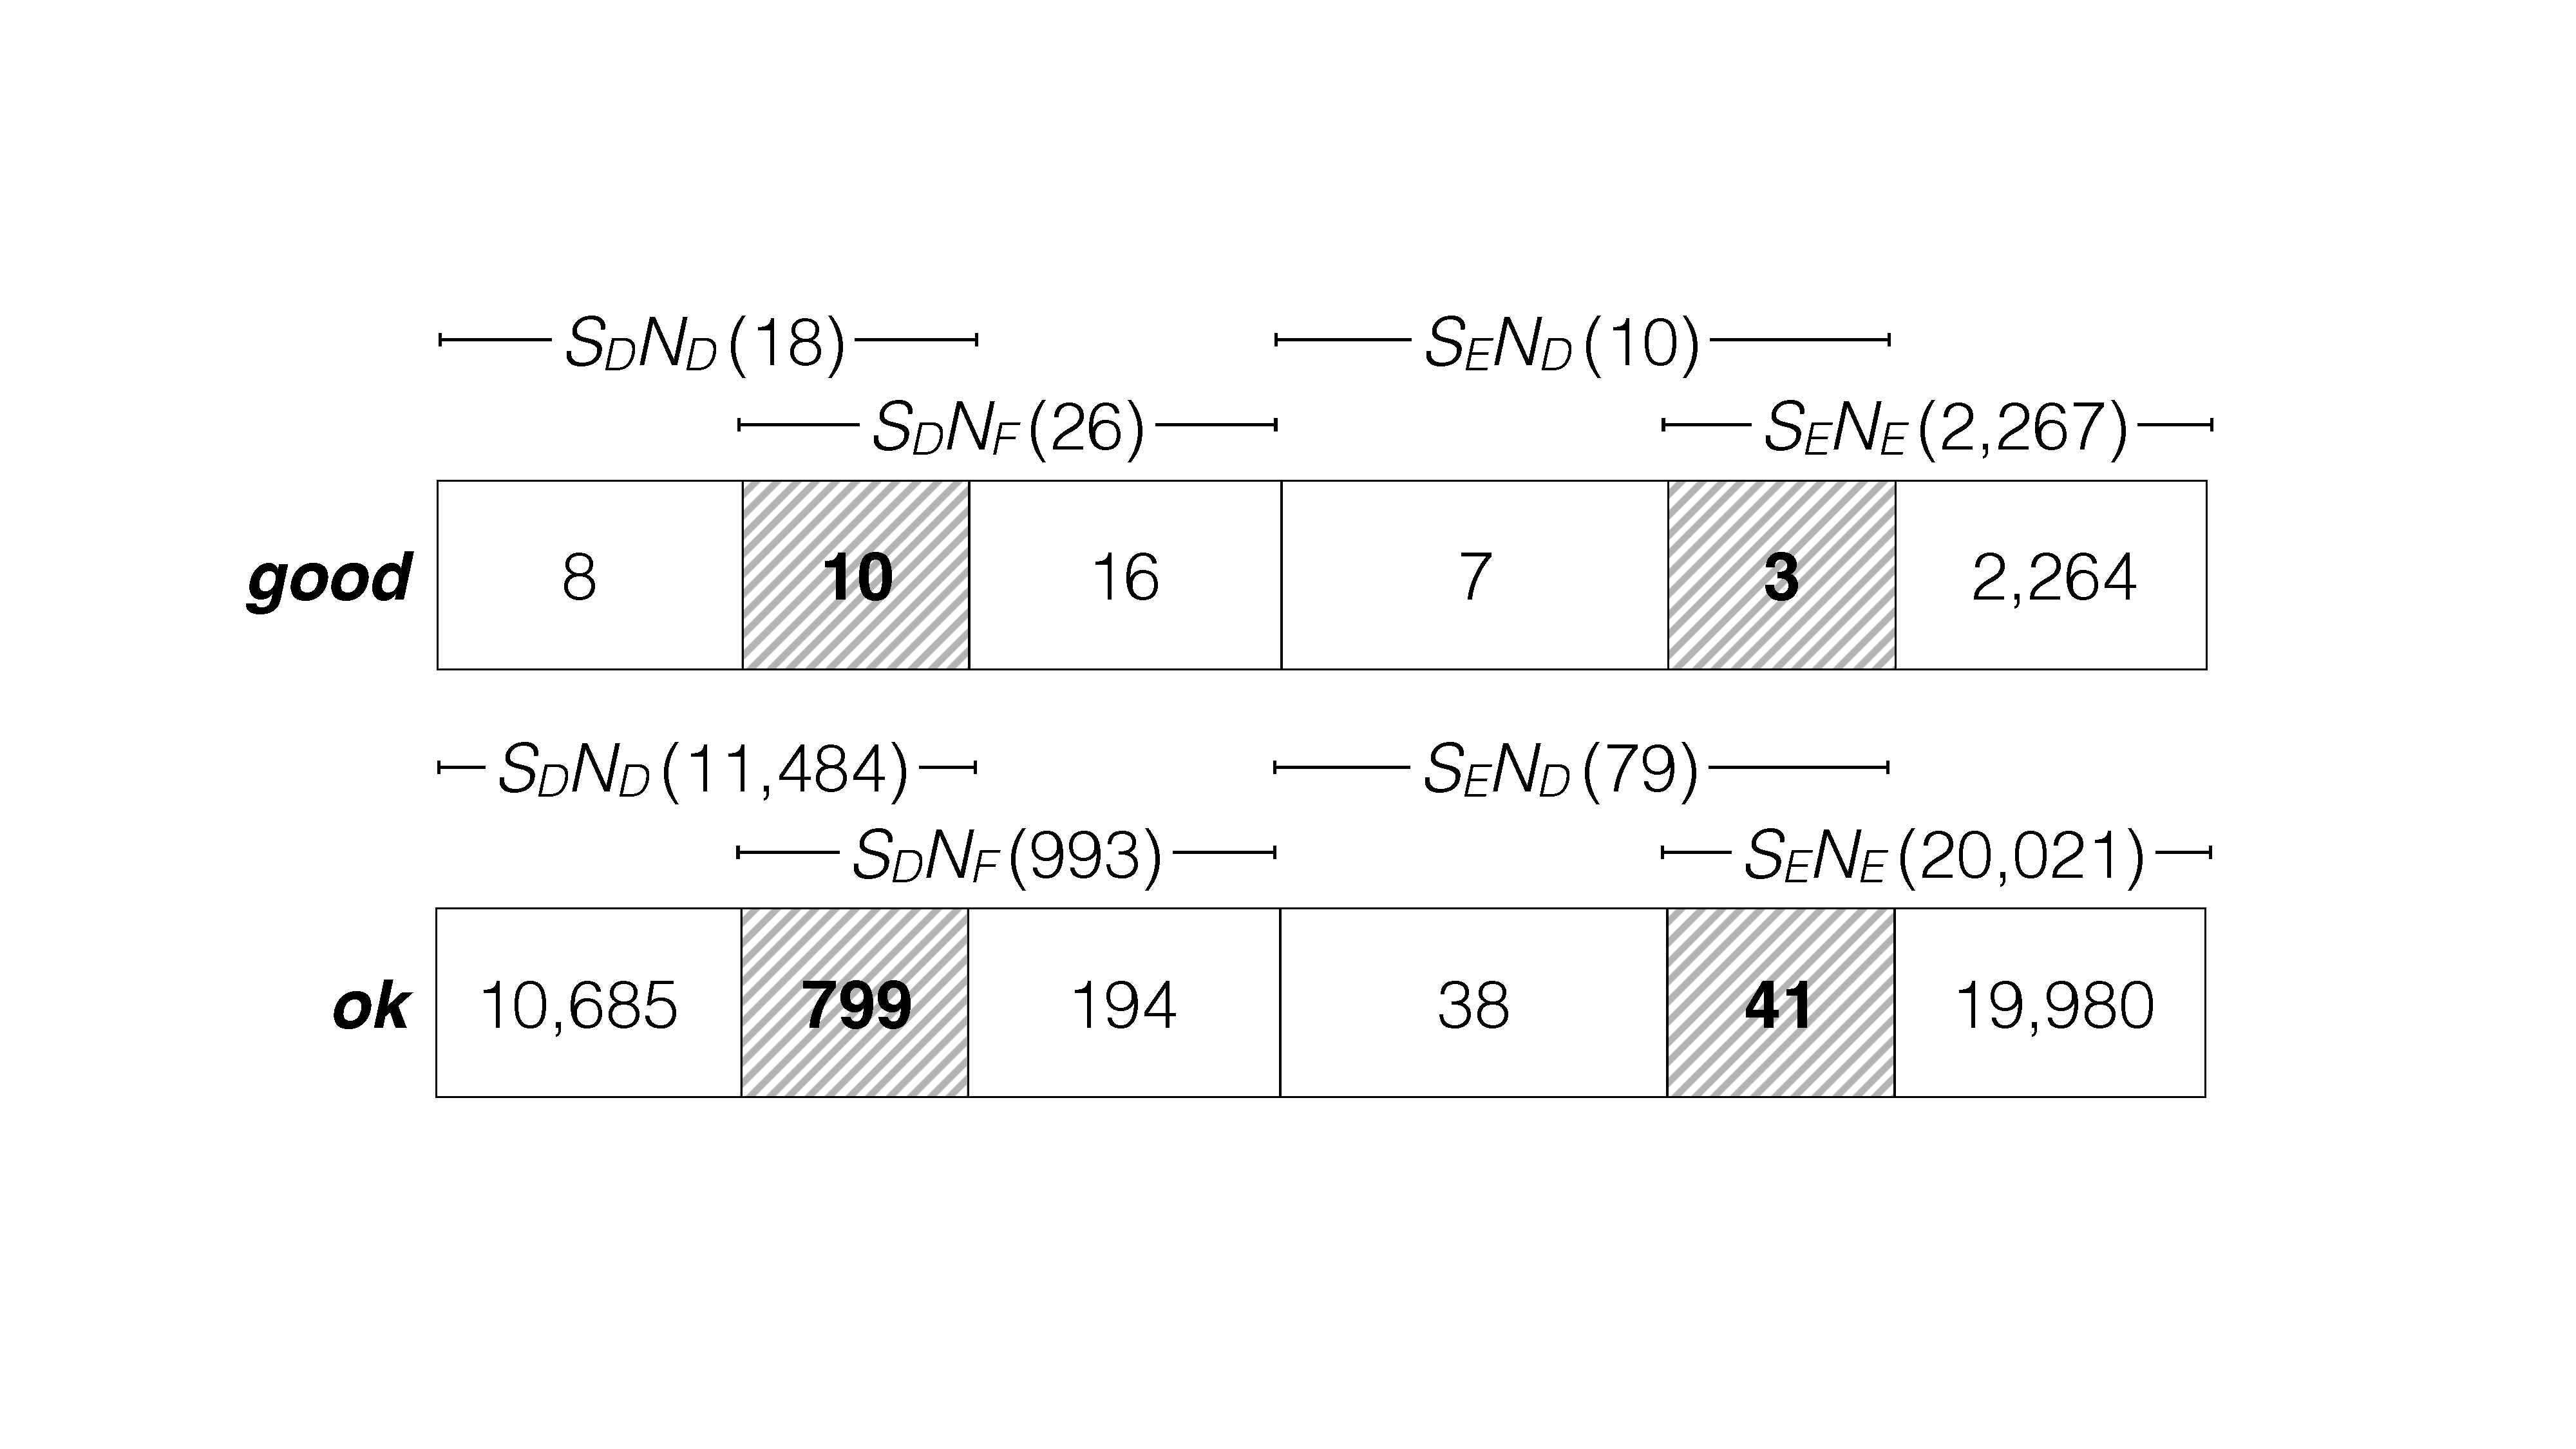
\includegraphics[width=\linewidth]{good-ok_pairs-crop}
	\caption{Distribution of \textit{good} (top) and \textit{ok} pairs (bottom) in 4 configurations of Simian and NiCad. The shaded areas are overlapping pairs.}
	\label{fig:good-ok-pairs}
\end{figure}

The distributions of \textit{good} clone pairs between four combinations of \textit{D} and \textit{E} configurations are listed in \Cref{t_agreed_good_clone_pairs} and depicted visually in \Cref{fig:good-ok-pairs}. There are 2,321 (2,308 unique) \textit{good} pairs consisting of 18 pairs from $S_DN_D$, 26 pairs from $S_DN_E$, 10 pairs from $S_EN_D$, and 2,267 pairs from $S_EN_E$. There are 32,560 (11,749 unique) \textit{ok} pairs\footnote{This excludes the subsumed 2,308 \textit{good} pairs. According to the definition, \textit{ok} pairs always subsume \textit{good} pairs.} We obtained 11,467; 993; 79; and 20,021 pairs from $S_DN_D$, $S_DN_E$, $S_EN_D$, and $S_EN_E$ respectively. Between the four configuration sets, there are considerable amount of clone pairs shared between two adjacent sets (as depicted in \Cref{fig:good-ok-pairs}), but there is no clone pair that is agreed by all four combinations. 

\subsubsection{Disagreed clone pairs}

The disagreed clone pairs are clone pairs that are reported by a single tool, either Simian or NiCad, and do not have agreement with clones from another tool. The disagreement can be from misalignment of clone lines or totally dissimilar clones due to different configurations. Disagreed pairs from Simian also cover clone pairs in projects having NiCad's errors (1 projects for $N_D$ and 5 for $N_E$) that are automatically missing from the agreed clone pairs. With the four configuration combinations, we decided to investigate only $S_D$, and $N_D$, and drop $S_E$ and $N_E$ due to their enormous amount of clone pairs (60 and 250 millions respectively). Moroever, without clone agreement, $S_E$ and $N_E$ contain a large number of false positives due to the recall preference of their EvaClone configurations. 

Even choosing only the default configurations, the number of clone pair candidates are still very large for manual inspection (67,570 for $S_D$ and 229,176 pairs for $N_D$). We hence apply four filters: \textbf{clone size, regular expression, similarity threshold, and good/ok pairs}. For the clone size filter, we raise the minimum clone size to 10 line as larger clones tend to be more interesting while smaller ones tend to be false clones~\cite{Saini2016}. Moreover, Gabel and Su show that unique code tend to be larger than seven lines~\cite{Gabel2010}. The 10--line threshold is already the default configuration for NiCad, thus this filter affects Simian clones only (Simian's default configurations consider a minimum of 6 lines).~The regular expression filter captures uninteresting boiler-plate clones of \verb|hashCode()| methods and some of the obvious getters and setters using regular expressions and removes them. The third filter, similarity threshold, applies only to NiCad clone pairs since Simian does not provide this similarity threshold configuration. The last filter, good/ok pairs, filters the pairs that already exist in \textit{good} or \textit{ok} set to avoid duplicates. 

As shown in \Cref{tab:online_clone_pairs}, for $S_D$ we filtered the results using clone size, regular expressions, and gook/ok pairs. The combination of the three filters reduce the number of $S_D$ clones to 17,801 pairs for manual investigation. 
For $N_D$, 10-line threshold is already a minimum NiCad's clone size. However, NiCad still reported much more clone pairs than Simian since it can detect type-3 clones. Thus, besides regular expressions and good/ok pair filters, we filtered NiCad's clones further by a stricter similarity threshold. We increase NiCad's similarity threshold from 70\% to 85\% (by adjusting NiCad's $\mathrm{UPI}$ from 0.3 to 0.15). We have tried varying the UPI from 70\% (default), 80\%, 85\% and 90\% and we found that 85\% similarity provides the best balance in terms of the amount of reported clones and feasibility for manual investigation. Using the three filters, we reduced the size of $N_D$ clones to 88 pairs.

In our clone classification process, we used a script to automatically classify {\small\texttt{equals()}} clone pairs which helped classifying 28,444 pairs out of 31,946 (more than half of the {\small\texttt{equals()}} pairs came from \textit{ok} and $S_D$ pairs). Finally, there are 3,502 pairs remaining which we manually classified them. The classification summary is shown in \Cref{tab:online_clone_classification_results}.

\textbf{To answer RQ1, we found 31,946 clone candidates between 111 Qualitas projects and 144,075 Stack Overflow snippets. They are 2,308 \textit{good}, 11,749 \textit{ok}, 17,801 $S_D$, and 88 $N_D$ pairs. After classification, we found 668 non-trivial online code clones pairs between Stack Overflow and Qualitas or external sources.}

\subsection{RQ2: Patterns of Online Code Cloning}

\begin{table}
	\centering
	\caption{Seven patterns of online code cloning}
	\label{tab:classification_scheme}
	\resizebox{\columnwidth}{!}{%
		\begin{tabular}{c|p{8.4cm}}
			\hline 
			Patt. & Descriptions \\ 
			\hline 
			QS & Cloned from Qualitas project to Stack Overflow (Q $\rightarrow$ S). \\ 
			\hline 
			SQ &Cloned from Stack Overflow to Qualitas project (S $\rightarrow$ Q). \\ 
			\hline 
			UD & Cloned from each other or from an external source \textit{X} outside the project (unknown) (S $\leftrightarrow$ Q $\vee$ (X $\rightarrow$ S $\wedge$ X $\rightarrow$ Q)).
			\\ 
			\hline 
			EX & Cloned from an external source (X $\rightarrow$ S $\wedge$ X $\rightarrow$ Q).
			\\ 
			\hline 
			BP & Boiler-plate or IDE auto-generated
			\\ 
			\hline 
			IN & Inheritance, interface implementation 
			\\ 
			\hline 
			AC & Accidental similarity, false clones \\ 
			\hline 
		\end{tabular}  %
	}
\end{table}

Besides the quantitative analysis, we are also interested in a qualitative analysis of the online clones. How are the clone pairs created? %Due to an absence of clone oracle of the two data sets, we resort to a manual investigation to classify the clone pair candidates using our 7 patterns of online code cloning.  

We started by a preliminary study of the 8 patterns of cloning from Kapser et al.~\cite{Kapser2006,Kapser2008}. This preliminary investigation aims to evaluate the applicability of Kapser's cloning patterns to our study. Using $S_D$ clone report, snippets are ranked according to (1) frequency, (2) popularity (i.e.~number of associated Qualitas projects), (3) clone size in SLOC, and (4) clone percentage compared to the snippet size. We selected these criteria so that we can cover clones across various aspects. We then picked the top 10 snippets from the 4 groups resulting in 34 unique Stack Overflow snippets chosen. The 34 snippets generate 697 clone pairs with Qualitas projects. Using Kapser's cloning patterns, the clone pairs were categorised into either Customisation or Templating. \textbf{Clearly Kapser's cloning patterns are too broad for our study and a more suitable and fine-grained classification scheme is needed.} 

Nevertheless, we adopted one of Kapser's cloning patterns, boiler-plate code and API/library protocol as pattern BP. We then added 6 new patterns observed as common cloning patterns from our preliminary study. The seven patterns include QS, SQ, UN, ES, BP, IN, and FC as presented in \Cref{tab:classification_scheme}. QS (\textbf{Q}ualitas to \textbf{S}tack Overflow) represents clones that has evidence to be copied from Qualitas to Stack Overflow (by having comments in source code and explanation/links in Stack Overflow post). Pattern SQ (\textbf{S}tack Overflow to \textbf{Q}ualitas) is the opposite of QS. UD (\textbf{U}nknown \textbf{D}irection) is cloning that creates exactly identical or highly similar clones but without any attribution of copying. They are unique enough not be boiler-plate and inheritance or interface implementation. ES (\textbf{Ex}ternal Sources) is a cloning that has an evidence of copying from an external source(s). Pattern BP (\textbf{B}oiler-\textbf{P}late) represents clones containing boiler-plate code of {\small\verb|equals()|} methods, getters and setters, or IDE-generated code (e.g.~GUI components). Pattern IN (\textbf{In}heritance/Interface) is cloning because of inheritance of the same super class or implementation of the same interface. They usually share similar overriding methods. The last pattern, AC (\textbf{A}ccidental \textbf{C}lones), represents false clone pairs. They can be either accidentally similar clones (e.g.~similar {\small\texttt{try-catch}} statements), similar clones after code normalisation, or just false positives of the tools. Using the classification patterns, we can also calculate the number of true and false positives. We are looking for unique and meaningful clones in this study. Thus, we consider clone pairs classified into pattern QS, SQ, UD, and EX as true positive, and BP, IN, and AC as false positive.

\subsubsection{Classification of Clone Candidates}

There were 31,946 online clone pair candidates for classifications as shown in \Cref{tab:online_clone_pairs}. We have use regular expressions to automatically classify \texttt{equals()}, getter and setter methods  based on the method signature since they are trivial clones and not very interesting. As shown in \Cref{tab:online_clone_classification_results}, the automatic classifier helped us captured 28,314 clone pairs and classified them into pattern BP. There were 3,632 pairs left for manual check after the automatic classification.

The first author who has been working on clone detection research for two years took the role of a main investigator performing a manual classification of all the 3,632 clone pairs. By consulting the cloning patterns, the main investigator manually went through each clone pair candidate, looked at the clones, and chose the most appropriate cloning pattern for the pair. A relevant and useful observation was also recorded for each clone pair. 

\begin{figure}
	\centering
	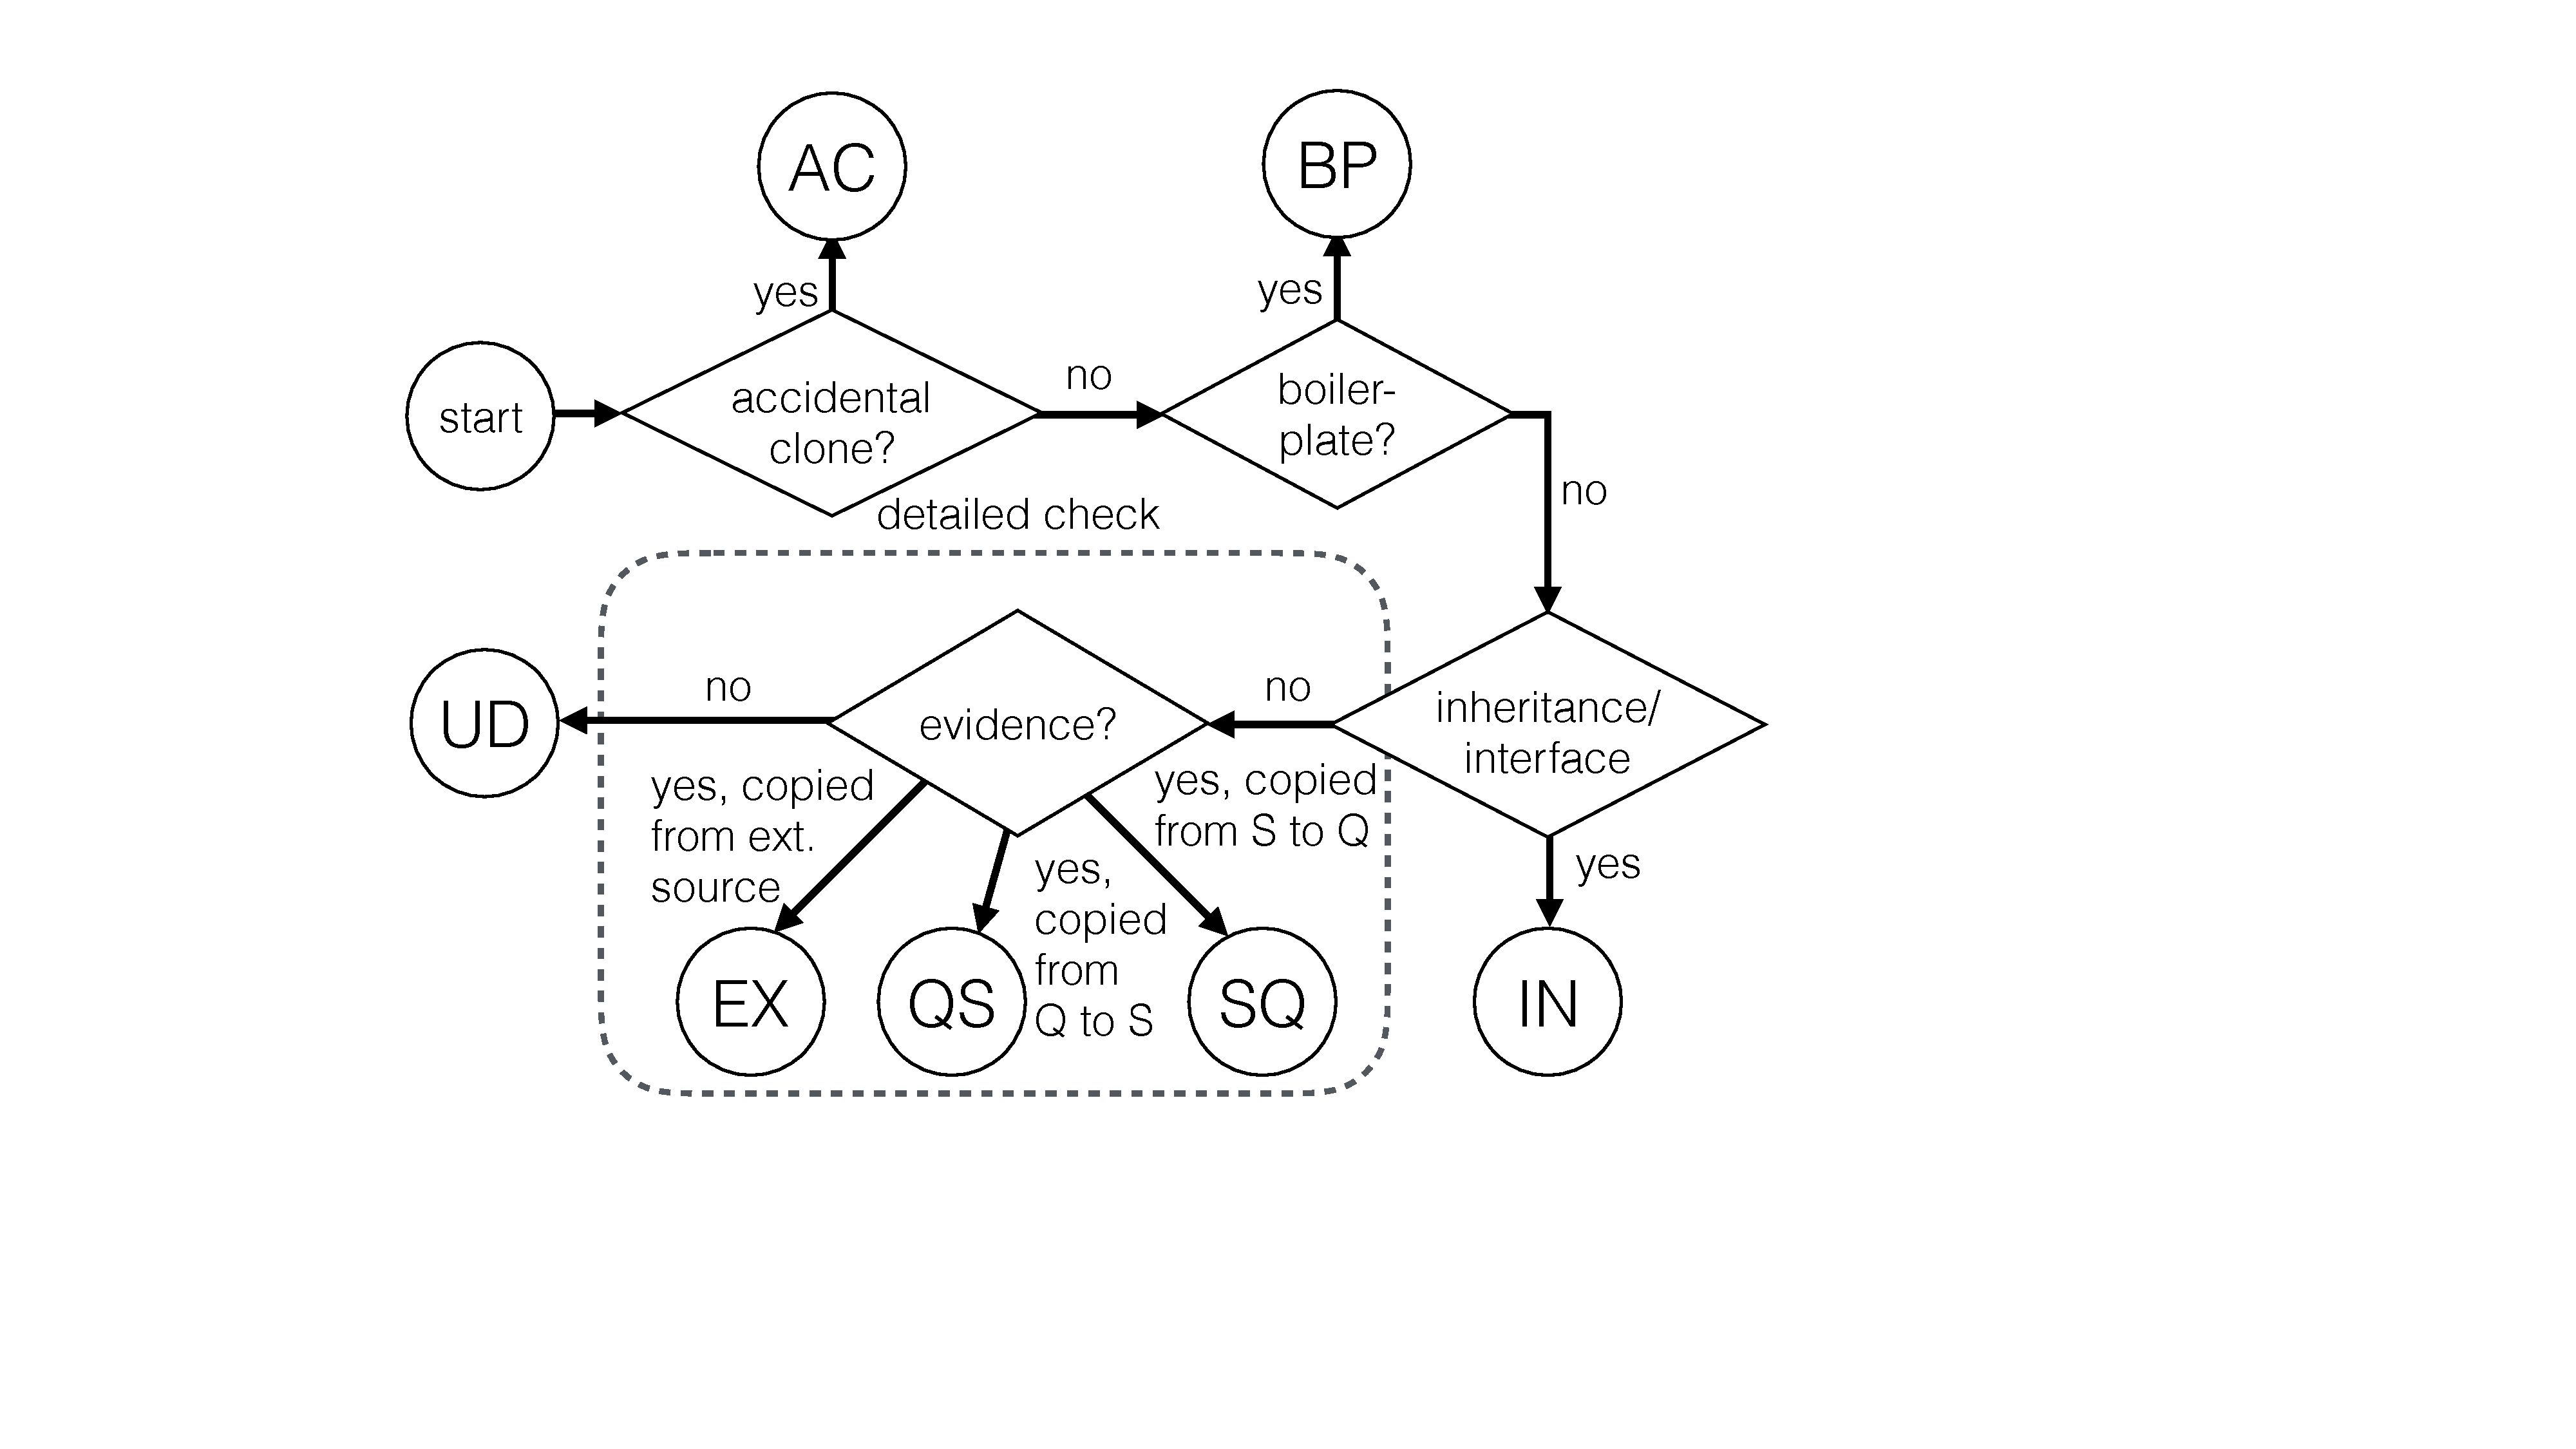
\includegraphics[width=0.8\linewidth]{classification_process}
	\caption{Online code clone classification process}
	\label{fig:classification_process}
\end{figure}

The investigator followed the following steps to classify the clones (depicted in \Cref{fig:classification_process}). First, we looked at the source code to see their similarity. If they were accidentally similar after code normalisation or by relaxation of the clone detection tool's configurations, the pair was classified as AC. If they were boiler-plate code, the pair was classified as BP. If they implemented the same interface or inherited the same class and had similar code, the pair was classified as IN. If the pair was not UD, IN, or AC; we started a detailed investigation. The main investigator opened the Stack Overflow post using its post ID with a web browser, read through the post carefully both in natural text and source code, looked for any hints or evidence mentioning code copying. If an evidence(s) had been found and appeared to be a Qualitas project as reported in the clone pair, the pair was classified as QS. Several times questions, name of posters, tags were also considered to gain better understanding. If there was no evidence on Stack Overflow but on Qualitas project mentioning about copying from Stack Overflow, the pair was classified as SQ. If there was evidence(s) of copying, but from an external source(s) instead of Qualitas, the pair was classified as EX. Lastly, if there was no evidence of copying in any direction, but source code of the clone pair are almost identical or highly similar, we conservatively classified them as UD.
  
To guarantee quality of the classification, the second author took the role of a validating investigator performing 10\% validation (363 pairs) of the clone pairs judged by the main investigator. After the validation, results from the two investigators were compared and 54 conflicts were found. The two investigators discussed and resolved 51 of them while 3 conflicts were resolved by the third author. The classification results are shown in \Cref{tab:classification_good_o}. 

\textbf{As an answer to RQ2, the classification results are explained and discussed below.}

\textbf{QS: Qualitas $\rightarrow$ Stack Overflow.} We found 110 online clone pairs with strong evidences of cloning from Qualitas projects to Stack Overflow. They include 3, 12, 86, and 9 pairs from \textit{good}, \textit{ok}, $S_D$, and $N_D$ set respectively. Most of them had statements in the Stack Overflow post saying that the code was ``copied'', ``modified'', ``adopted'' from a specific file or class in Qualitas. The most cloned projects were \texttt{hibernate} and \texttt{spring} having 20 clone pairs, followed by \texttt{eclipse} (15), and \texttt{hadoop} (12). The clones were mostly cloned as examples and were very similar to their original Qualitas code with limited modifications.

\textbf{SQ: Stack Overflow $\rightarrow$ Qualitas.} We did not find any clone pairs with strong evidences of cloning from Stack Overflow to Qualitas projects.

\textbf{UD: Unknown Direction.} We found 382 online clone pairs with no evidence of cloning between Qualitas and Stack Overflow but with high code similarity. They include 11, 42, 294, and 35 pairs from \textit{good}, \textit{ok}, $S_D$, and $N_D$ set respectively. The most cloned projects in this pattern was {\small{\texttt{netbeans}}} which had 95 clone pairs. Most of the clones were large chunk of code involving GUI components which might also be auto-generated. However, we also did not have any evidence. The second most cloned project was {\small{\texttt{jung2}}} (62 pairs) that was a network and graph framework. There were several Stack Overflow snippets that were identical to code in {\small{\texttt{jung2}}}. The third project was {\small{\texttt{eclipse-SDK}}} (37 pairs).

\textbf{EX: External Sources.} We found 178 online clone pairs with evidences of cloning from external sources to Stack Overflow. They include 4, 23, 145, and 6 pairs from \textit{good}, \textit{ok}, $S_D$, and $N_D$ set respectively.
%\begin{table}[]
%	\centering
%	\caption{31 external clones found in Stack Overflow posts}
%	\label{tab:ext_clones}
%	\begin{tabular}{l|r|r}
%		\hline
%		Type        & FOSS & Web \\ \hline
%		StackOverflow only     & 1    & 1   \\
%		StackOverflow + Qualitas & 15   & 14  \\ \hline
%	\end{tabular}
%\end{table}
This findings complement a study of inter clones between software projects~\cite{Svajlenko2014}. We show that, besides software projects, clones can also be copied over different websites on the Internet. There are 15 clone pairs that are originated from programming websites. For example, we found a clone of code snippet to convert numbers into words which is copied from www.rgagnon.com/javadetails/java-0426.html. Both Stack Overflow and {\small\texttt{compiere}} project source code contain attribution to the original source. Another example is a code of algorithm to generate graphical \textit{Perlin noise} copied from http://mrl.nyu.edu/\textasciitilde perlin/noise/. This code is used in both Stack Overflow and {\small\texttt{aoi}} project with attribution. %The original code of the 15 clone pairs do not have licensing information so these clones do not violate any license. 
There were 12 pairs cloned from {\small\texttt{zxing}}, {\small\texttt{jasper}}, {\small\texttt{java.util}}, {\small\texttt{javax.servlet}}, and {\small\texttt{org.bouncycastle.crypto}} project.

\textbf{BP: Boiler-Plate.} There were a large amount of boiler-plate clone pairs found in this study. Although we surly removed some of the boiler-plate code with filters before the analysis, we still observed 28,642 BP clone pairs which accounted for 89.7\% of all clone pairs we classified. The majority of them were {\small{\texttt{equals()}}} methods.

\textbf{IN: Inheritance/interface.} There were 109 clone pairs found to be similar because they implemented the same interface or inheriting from the same class. An example was two implementations of {\small{\texttt{MouseListener}}} that share similar {\small\texttt{@Override}} methods of {\small\texttt{mousePressed}}, and {\small\texttt{mouseReleased}}. 

\textbf{AC: Accidental Clones.} 31,946 were clone pairs that were accidentally similar due to several reasons. Mainly, they were caused by the effects of code normalisation applied to the source code before detection. However, the original source code were still different enough when we manually classified them. Other causes include {\small\texttt{finally}} or {\small\texttt{try-catch}} clauses that were accidentally the same due to their very small sizes, or clearly non-cloned code which may somehow miss the tools' detections.

%For \textit{good} pairs, 10 pairs were automatically classified by regular expressions and 2,298 pairs were manually classified. This resulted in 3 clone pairs in pattern QS which is found to be copied from a Qualitas project to Stack Overflow. Four pairs are highly similar or identical but without any evidence of copying (no comments in neither Stack Overflow post nor Qualitas source code) and are classified as pattern UD. Please note that we were conservative in this study when doing classification. Even the clone pairs were exactly or almost identical but we could not find an evidence that it was cloned in any particular direction, we classified them as UD instead of QS, SQ, or EX. We observed 4 pairs in pattern EX since they are copied from external sources. 111 clone pairs are found to be pattern BP. Seven pairs are similar code from inheriting the same superclass or implementing the same interface, pattern IN. Finally, 2,172 pairs are false clones and classified into FC. No clones were found in pattern SQ. This was expected since we selected a pretty old Qualitas snapshot dated back 2013 and most of the code could be written long before that.  

%For \textit{ok} clone pairs, we could not feasibly investigate all 31,729 pairs manually and decided to remove $S_EN_E$ from this round of classification. According to the classification of \textit{good} pairs, we found that $S_EN_E$ accounted for 98.9\% of all false positive pairs in \textit{good} pairs. This was not a surprise since EvaClone configurations prefered recall and hence offered relaxed configurations. We ignored them since we were more interested in meaningful clones. This resulted in 11,749 \textit{ok} pairs remaining. 11,494 clone pairs were automatically classified and 255 pairs were looked at manually. 
%We found 12, 42, 23, 11,459, 20, and 103 in QS, UD, EX, BP, IN and AC respectively. Similarly, no clone pairs were found in SQ. 

\begin{table}
	\centering
	\caption{Classification results of agreed and disagreed clone pairs.}
	\label{tab:classification_good_o}
	\small
	\resizebox{\columnwidth}{!}{%
		\begin{tabular}{l|r|r|r|r|r|r|r|r}
			\hline
			Set & QS & SQ & UD & EX & BP & IN & AC & Total \\ 
			\hline
			\multirow{1}{*}{\textit{good}}  & 3 & 0 & 11 & 4 & 111  & 7 & 2,172 & 2,308 \\
			\multirow{1}{*}{\textit{ok}}  & 14 & 0 & 20 & 41 & 11,547 & 22 & 105 & 11,749 \\
			\multirow{1}{*}{$S_D$} & 86 & 0 & 293 & 146 & 17,074 & 74 & 128 & 17,801 \\
			\multirow{1}{*}{$N_D$} & 9  & 0 & 35 & 6 & 17 & 8 & 13 & 88 \\ 
			\hline
			Total & 112 & 0 & 359 & 197 & 28,749 & 111 & 2,418 & 31,946 \\ 
			\hline
		\end{tabular} 
	}
\end{table}

%For 17,801 $S_D$ clone pairs, they contained a large volume of boiler-plate code. Our regular expressions could automatically classified 16,800 of them into BP. The investigator checked the 1,001 remaining pairs manually. As a result, we found 86 QS, 294 UD, 145 EX, 17,074 BP, 74 IN and 128 AC pairs. For 88 $N_D$ clone pairs, 10 of them were automatically classified into BP and 78 were manually classified. We found 9 QS, 35 UD, 6 EX, 17 BP, 8 IN, and 13 AC respectively.

%\textbf{We answer RQ2 by using our patterns of online code cloning to classified 31,946 clone pairs. We found that a large amount of the clone pairs are boiler-plate code (28,642), clones from inheritance/interface (109), or accidental clones (2,525). Nevertheless, there were 670 pairs that were intentionally created. 110 pairs had strong evidences to be cloned from Qualitas to Stack Overflow. 382 were highly-confident clones but without evidence of cloning direction. 178 pairs were found to be cloned from external sources outside Qualitas projects.} %We did not find any clone pairs in the direction from Stack Overflow to Qualitas.}

\subsection{RQ3: Outdated Online Code Clones}

%In this study, we are interested in effects of having code clones between open source software systems and Stack Overflow. From the manual investigation, we found 523 true positive online clone pairs. With this set of true clones, we investigated further and found that there are two potential issues, outdated code and software licensing violation.

%\subsubsection{Outdated Clones}
To the best of our knowledge, this work is the first to discuss a problem of outdated code on Stack Overflow. Outdated code occurs when a piece of code has been copied from its origin to another location and later the original code has been updated~\cite{Xia2014}. Usually code clone detection is used to locate clone instances and update them to match with the original code~\cite{Bellon2007}. However, for online code clones, the clones are pervasive and are more difficult to detect than in a local project(s) due to its large search space and the mix of natural and programming language combined together in Stack Overflow posts. Moreover, Stack Overflow is not a software. There is no test suite to run and check whether the code snippets are still working as expected.

To check if our online code clones are outdated, we focused on the 112 QS clone pairs that were cloned from Qualitas to Stack Overflow (see \Cref{tab:classification_good_o}) and compared them with their latest versions. We cloned the latest version of the Qualitas projects from their repositories on 26 September 2016. For each online clone pair, we used the file name of Qualitas clone to search for its latest version. Once we found the file, we located the location of the cloned snippets in the file based on method names. So for Simian clones that may not contain in a single method, we looked further up and down the clone region to get the method name and its nearby methods. We then compared the Stack Overflow snippet to its latest version line-by-line to find if any change has been made to the source code. We also made sure that the changes did not come from modifications maded to Stack Overflow snippets by the posters but from the projects themselves. When we found inconsistent lines between the two versions, we used \texttt{git blame} command to see who modified those lines of code and noted down the details.

\Cref{fig:outdated} shows the findings of outdated online clones on Stack Overflow. We discovered 64 outdated online clone pairs out of 112 pairs. {\small{\texttt{spring}}} and {\small{\texttt{hibernate}}} have the maximum number of 20 outdated pairs, followed by 15 from {\small{\texttt{eclipse}}}, and 12 from {\small{\texttt{hadoop}}}. An example of outdated code in {\small{texttt{hadoop}}}'s {\small{\texttt{WritableComparator.java}}} has already been shown in \Cref{fig:before-after}. We also found a few outdated code which contained heavy modifications. For example, the code snippet in Stack Overflow post 23520731, a copy of {\small{\texttt{SchemaUpdate.java}}} in {\small{\texttt{hibernate}}}, it had been heavily modified in the latest version (as shown in \Cref{fig:hibernate_outdated_code}). In the 64 outdate pairs, we found 5 of them to be ``dead'' snippets. These snippets did not have their originals in the latest version of the projects anymore. For example, the snippet in Stack Overflow post 3758110, a copy of {\small{\texttt{DefaultAnnotationHandlerMapping.java}}} in {\small{\texttt{spring}}}, was deleted in commit {\small{\texttt{02a4473c62d8240837bec297f0a1f3cb67ef8a7b}}} by Chris Beams on 20th January 2012 at 22:51:02, two years after it was posted. %The latest version of Spring does not contain the file anymore. 

The outdated online code clones can cause problems ranging from uncompilable code (due to modifications and different API usage in the outdated code) to bug propagations. An outdated code with a subtle change (e.g.~\Cref{fig:before-after}) may be copied and reused without awareness from developers. Although Stack Overflow has a voting mechanism that may mitigate this outdated code issue, the check mark symbol in front of the accepted answer is still attractive enough for naive developers who are ignorant to copy and reuse the code.

\textbf{For RQ3, our results show that more than half (64) of QS clone pairs on Stack Overflow are outdated. 60 pairs differ from their newest versions by modifications applied to variable names or method names, added or deleted statements, to a fully rewritten code with new method signatures. 4 pairs are dead snippets. They do not exist any more in the latest version. These outdated Stack Overflow online clone snippets are questionable for reuse.} %These changes did not reflect They might later find out that the copied code does not work any more due to different API versions. Even worse, they might also introduce bugs or vulnerabilities into their software.  }
%Usually when developers reuse a code snippet from a Stack Overflow post and find that it does not work nor compatible with their environment. They can cast a down vote to that answer resulting in low votes for the answer (which might be outdated). However, if the answer is marked as accepted by the person who asks the question, the check mark symbol attached to the answer is still attractive to naive developers who are ignorant. 

\begin{figure*}
	\begin{lstlisting}
          /* Code in Stack Overflow #23520731 */             /* SchemaUpdate.java (2016-09-26) */
          public void execute (Target target) {              public void execute(EnumSet<TargetType> targetTypes, 
            LOG.runningHbm2ddlSchemaUpdate();                                Metadata metadata, ServiceRegistry serviceRegistry) {
            Connection connection = null;                      if ( targetTypes.isEmpty() ) {
            Statement stmt = null;                               LOG.debug(""Skipping SchemaExport as no targets were specified"");
            Writer outputFileWriter = null;                      return;
            exceptions.clear();                                }
            try {                                              exceptions.clear();
              DatabaseMetadata meta;                           LOG.runningHbm2ddlSchemaUpdate();
              ...                                              ...
	\end{lstlisting}
	\caption{Outdated code snippet on Stack Overflow post 23520731. This code has been copied from \texttt{SchemaUpdate.java} and its latest version in hibernate code base contains heavy modifications.}
	\label{fig:hibernate_outdated_code}
\end{figure*}

\begin{figure}
	\centering
	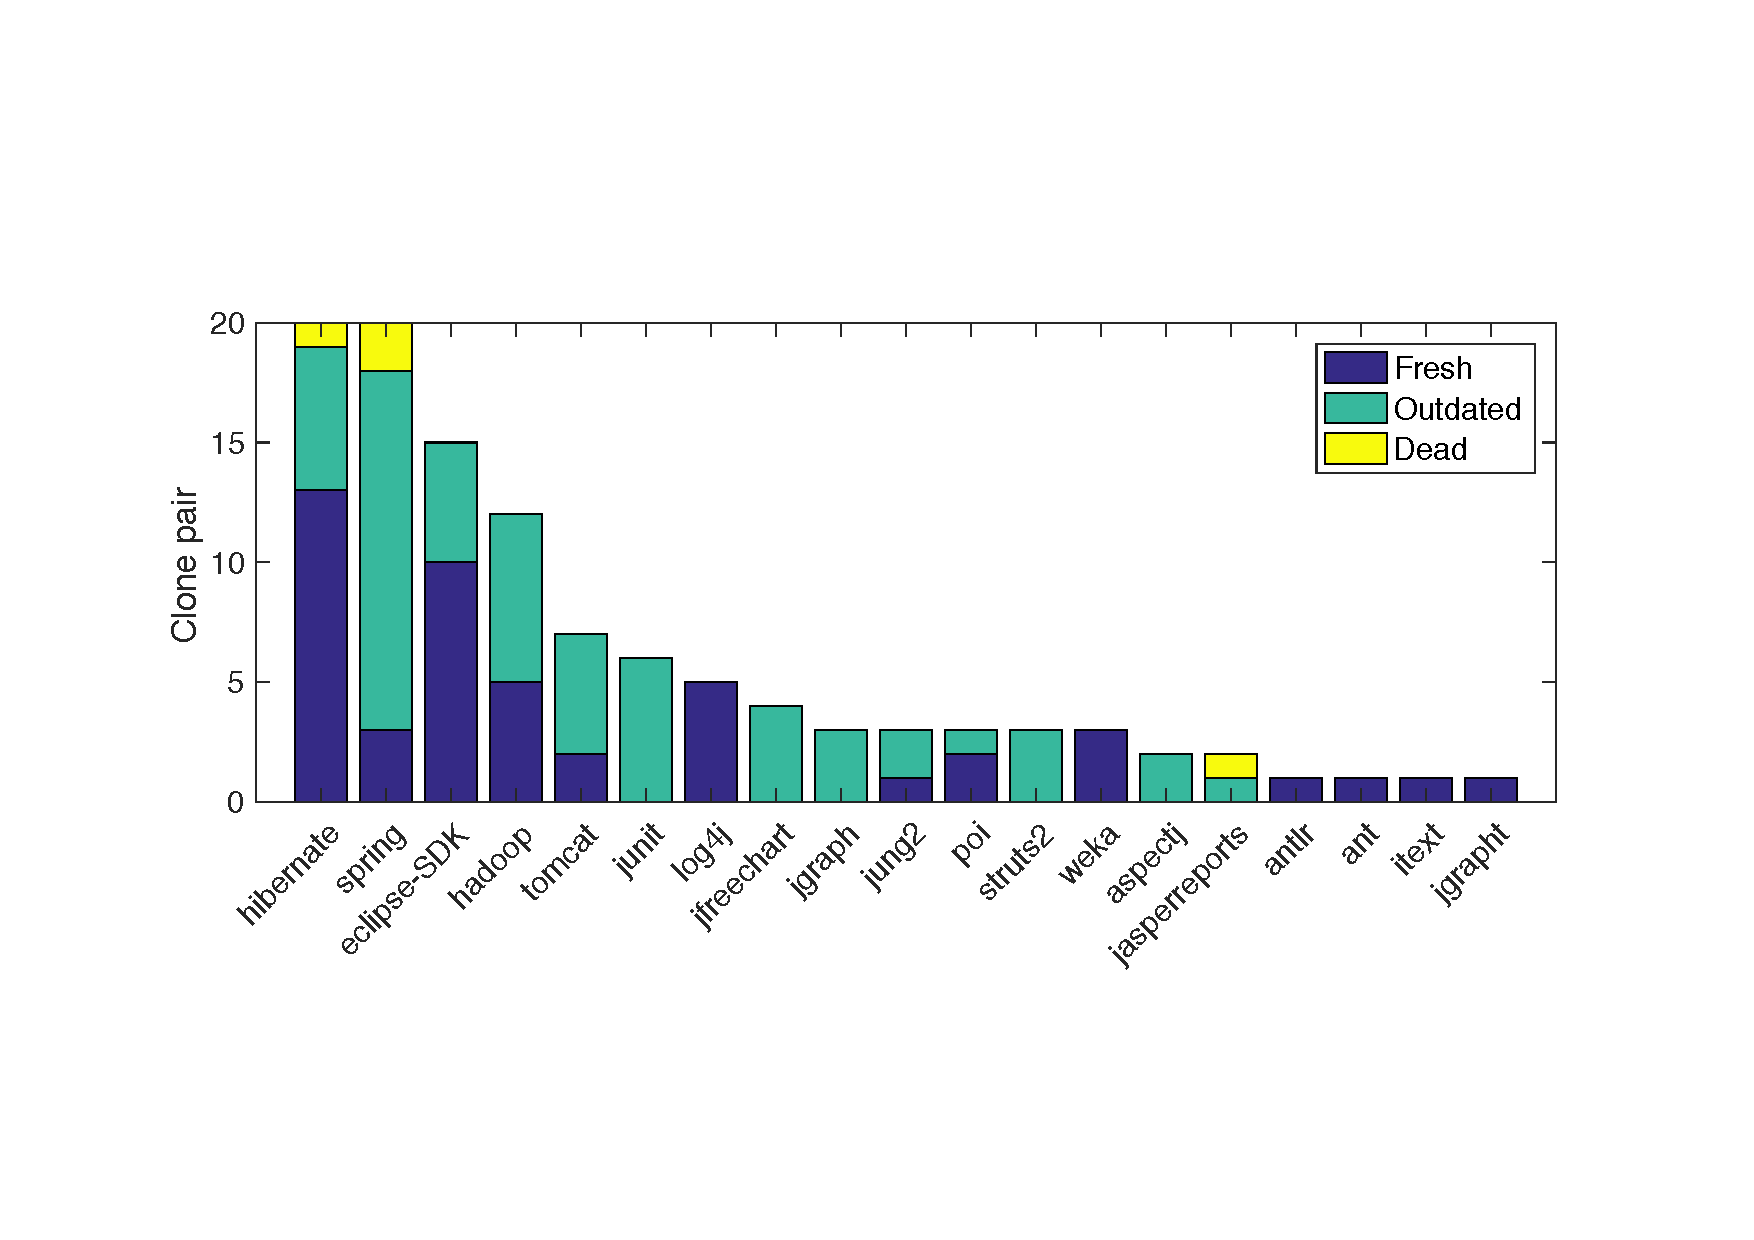
\includegraphics[width=\linewidth]{freshness}
	\caption{Freshness of 110 QS online clone pairs}
	\label{fig:outdated}
\end{figure}

\begin{table*}
	\centering
	\caption{62 QS outdated online clone pairs. Outdated clones are caused by modified/added/deleted statements (\textit{S}), file deletion (\textit{D}), and method rewriting (\textit{R}).}
	\label{tab:stale_code_details}
	\small
	\resizebox{2\columnwidth}{!}{%
	\begin{tabular}{r|l|l|l|l|p{5.2cm}|r|r|l|c|l}
		\hline 
		\multirow{2}{*}{No.} & \multicolumn{2}{c|}{Stack Overflow} & \multicolumn{6}{c|}{Qualitas} & \multicolumn{2}{c}{Changes} \\ \cline{2-11}
		& Post & Date & Project & Ver. & File & Start & End & Date & Type & Date \\
		\hline
			1 & 18303692 & 18-Aug-13 & aspectj & 1.6.9  & aspectjtools/../Agent.java & 7 & 18 & 5-Mar-08 & \textit{S} & 8-Sep-15 \\
			2 & 18303692 & 18-Aug-13 & aspectj & 1.6.9  & aspectjweaver/../Agent.java & 7 & 18 & 5-Mar-08 & \textit{S} & 8-Sep-15 \\
			3 & 2513183 & 25-Mar-10 & eclipse-SDK & 4.3 & GenerateToStringAction.java & 113 & 166 & 5-Jun-13 & \textit{S} & 17-Mar-15 \\
			4 & 2513183	& 25-Mar-10 & eclipse-SDK & 4.3 & GenerateToStringAction.java & 117 & 126 & 5-Jun-13 & \textit{S} & 17-Mar-15 \\
			5 & 2513183	& 25-Mar-10 & eclipse-SDK & 4.3 & GenerateToStringAction.java & 143 & 165 & 5-Jun-13 & \textit{S} & 1-Mar-11 \\
			6 & 2513183	& 25-Mar-10 & eclipse-SDK & 4.3 & GenerateToStringAction.java & 178 & 187 & 5-Jun-13 & \textit{S} & 5-Jun-13 \\
			7 & 11861598 & 8-Aug-12 & eclipse-SDK & 4.3 & WizardDialog.java & 377 & 394 & 1-May-13 & \textit{S} & 21-Jun-13 \\
			8 & 22315734 & 11-Mar-14 & hadoop & 1.0.0 & WritableComparator.java & 44 & 54 & 25-Aug-11 & \textit{S} & 20-Nov-14 \\
			9 & 801987 & 29-Apr-09 & hadoop & 1.0.0 & StringUtils.java & 40 & 56 & 15-Dec-11 & \textit{S} & 4-Feb-13 \\
			10 & 21702608 & 11-Feb-14 & hadoop & 1.0.0 & DBCountPageView.java & 275 & 287 & 15-Dec-11 & \textit{S} & 12-Jun-11 \\
			11 & 21702608 & 11-Feb-14 & hadoop & 1.0.0 & DBCountPageView.java & 289 & 309 & 15-Dec-11 & \textit{S} & 12-Jun-11 \\
			12 & 14845581 & 13-Feb-13 & hadoop & 1.0.0 & JobSubmissionFiles.java & 46 & 55 & 15-Dec-11 & \textit{S} & 25-Jun-12 \\
			13 & 16180910 & 24-Apr-13 & hadoop & 1.0.0 & mapred/../LineRecordReader.java & 47 & 60 & 15-Dec-11 & \textit{R} & 25-Jul-11 \\
			14 & 16180910 & 24-Apr-13 & hadoop & 1.0.0 & mapreduce/../LineRecordReader.java & 41 & 54 & 15-Dec-11 & \textit{R} & 25-Jul-11 \\
			15 & 15168494 & 24-Feb-14 & hibernate & 4.2.2 & ConnectionProviderInitiator.java & 65 & 93 & 22-May-13 & \textit{S} & 26-Apr-13 \\
			16 & 24924255 & 24-Jul-14 & hibernate & 4.2.2 & Example.java & 224 & 243 & 22-May-13 & \textit{S} & 23-Apr-13 \\
			17 & 23520731 & 7-May-14 & hibernate & 4.2.2 & SchemaUpdate.java & 115 & 168 & 22-May-13 & \textit{S} & 5-Feb-16 \\
			18 & 8257554 & 26-Nov-11 & hibernate & 4.2.2 & SettingsFactory.java & 244 & 255 & 22-May-13 & \textit{D} & 11-Mar-11 \\
			19 & 23967852 & 31-Apr-14 & hibernate & 4.2.2 & SQLServer2005LimitHandler.java & 43 & 61 & 22-May-13 & \textit{S} & 11-May-16 \\
			20 & 19298607 & 10-Oct-13 & hibernate & 4.2.2 & Oracle9iDialect.java & 23 & 32 & 22-May-13 & \textit{S} & 12-Apr-15 \\
			21 & 10031897 & 5-Apr-12 & hibernate & 4.2.2 & AliasToBeanResultTransformer.java & 44 & 61 & 22-May-13 & \textit{S} & 4-Jun-15 \\ 
			22 & 8037824 & 7-Nov-11 & jasperreports & 3.7.4 & JRVerifier.java & 982 & 998 & 31-May-10 & \textit{S} & 17-Apr-08 \\
			23 & 8037824 & 7-Nov-11 & jasperreports & 3.7.4 & JRVerifier.java & 1221 & 1240 & 31-May-10 & \textit{D} & 20-May-11 \\
			24 & 12936580 & 17-Oct-12 & jfreechart & 1.0.13 & AbstractXYItemRenderer.java & 532 & 569 & 20-Apr-09 & \textit{S} & 16-Jan-16 \\
			25 & 16058183 & 17-Apr-13 & jfreechart & 1.0.13 & KeyToGroupMap.java & 18 & 30 & 20-Apr-09 & \textit{S} & 29-Jun-07 \\
			26 & 21998949 & 24-Feb-14 & jfreechart & 1.0.13 & SpiderWebPlot.java & 502 & 520 & 20-Apr-09 & \textit{S} & 2-Jun-08 \\
			27 & 21998949 & 24-Feb-14 & jfreechart & 1.0.13 & SpiderWebPlot.java & 522 & 536 & 20-Apr-09 & \textit{S} & 22-Nov-13 \\
			28 & 6722760 & 17-Jul-11 & jgraph & 5.13.0.0 & HelloWorld.java (3 overlaps)  & 14 & 37 & 25-Sep-09 & \textit{R} & 13-Apr-14 \\
			31 & 6025026 & 17-Jul-11 & jung2 & 2\_0\_1  & ShortestPathDemo.java & 106 & 117 & 20-Jun-08 & \textit{S} & 13-Apr-10 \\
			32 & 6025026 & 17-Jul-11 & jung2 & 2\_0\_1  & ShortestPathDemo.java & 158 & 172 & 20-Jun-08 & \textit{S} & 29-Nov-15 \\
			33 & 23586872 & 31-May-14 & junit & 4.11 & Assert.java & 33 & 52 & 11-Oct-12 & \textit{S} & 12-May-15 \\
			34 & 7504040 & 29-Sep-11 & junit & 4.11 & ExternalResource.java (3 overlaps) & 4 & 23 & 11-Oct-12 & \textit{S} & 25-Jun-16 \\
			37 & 8802082 & 10-Jan-12 & junit & 4.11 & ExpectException.java (2 overlaps) & 11 & 29 & 11-Oct-12 & \textit{S} & 25-May-14 \\
			39 & 12593810 & 26-Sep-12 & poi & 3.6 & WorkbookFactory.java & 18 & 28 & 7-Dec-09 & \textit{R} & 26-Jun-13 \\
			40 & 20913543 & 6-Jan-14 & spring & 3.0.5  & AutowireUtils.java & 32 & 42 & 20-Oct-10 & \textit{S} & 28-Oct-14 \\
			41 & 18623736 & 4-Sep-13 & spring & 3.0.5  & CustomCollectionEditor.java & 33 & 71 & 20-Oct-10 & \textit{S} & 21-Nov-13 \\
			42 & 22865824 & 4-Apr-14 & spring & 3.0.5  & JavaMailSenderImpl.java & 169 & 185 & 20-Oct-10 & \textit{S} & 6-Oct-14 \\
			43 & 22865824 & 4-Apr-14 & spring & 3.0.5  & JavaMailSenderImpl.java & 186 & 197 & 20-Oct-10 & \textit{S} & 6-Oct-14 \\
			44 & 20421869 & 6-Dec-13 & spring & 3.0.5  & ClassPathScanningCandidateComponent\newline Provider.java (2 overlaps) & 85 & 133 & 20-Oct-10 & \textit{R} & 12-Aug-16 \\
			46 & 3751463 & 20-Sep-10 & spring & 3.0.5  & ScheduledTasksBeanDefinitionParser.java & 42 & 52 & 20-Oct-10 & \textit{S} & 21-May-12 \\
			47 & 6149818 & 27-May-11 & spring & 3.0.5  & DefaultPropertiesPersister.java & 69 & 80 & 20-Oct-10 & \textit{S} & 19-Mar-13 \\
			48 & 10952561 & 8-Jun-12 & spring & 3.0.5  & HibernateTemplate.java & 761 & 769 & 20-Oct-10 & \textit{S} & 9-May-15 \\
			49 & 10952561 & 8-Jun-12 & spring & 3.0.5  & Jaxb2Marshaller.java & 253 & 269 & 20-Oct-10 & \textit{S} & 28-Aug-12 \\
			50 & 20996373 & 8-Jan-14 & spring & 3.0.5  & test/../DelegatingServletInputStream.java & 6 & 20 & 20-Oct-10 & \textit{S} & 18-Dec-08 \\
			51 & 20996373 & 8-Jan-14 & spring & 3.0.5  & web/../DelegatingServletInputStream.java & 6 & 20 & 20-Oct-10 & \textit{S} & 15-Jul-16 \\
			52 & 20996373 & 8-Jan-14 & spring & 3.0.5  & servlet/../ DelegatingServletInputStream.java & 6 & 20 & 20-Oct-10 & \textit{S} & 15-Jul-16 \\
			53 & 5660519 & 15-Apr-11 & spring & 3.0.5 & AnnotationMethodHandlerException\newline Resolver.java & 224 & 233 & 20-Oct-10 & \textit{D} & 20-Jan-12 \\
			54 & 4781746 & 24-Jan-11 & spring & 3.0.5  & DispatcherServlet.java & 91 & 103 & 20-Oct-10 & \textit{S} & 8-Aug-11 \\
			55 & 3758110 & 21-Sep-10 & spring & 3.0.5  & DefaultAnnotationHandlerMapping.java & 78 & 92 & 20-Oct-10 & \textit{D} & 20-Jan-12 \\
			56 & 9003314 & 25-Jan-12 & spring & 3.0.5  & WebDataBinder.java & 95 & 108 & 20-Oct-10 & \textit{S} & 15-Aug-10 \\
			57 & 14019840 & 24-Dec-12 & struts2 & 2.2.1  & DefaultActionMapper.java & 128 & 144 & 17-Jul-10 & \textit{S} & 18-Oct-13 \\
			58 & 15131432 & 28-Feb-13 & struts2 & 2.2.1  & FreemarkerManager.java & 163 & 177 & 17-Jul-10 & \textit{S} & 28-Oct-13 \\
			59 & 15110171 & 27-Feb-13 & struts2 & 2.2.1  & StringLengthFieldValidator.java & 25 & 42 & 17-Jul-10 & \textit{S} & 15-Jun-15 \\
			60 & 21734562 & 12-Feb-14 & tomcat & 7.0.2  & BasicAuthenticator.java (2 overlaps) & 25 & 73 & 4-Aug-10 & \textit{R} & 4-Aug-16 \\
			62 & 21734562 & 12-Feb-14 & tomcat & 7.0.2  & FormAuthenticator.java & 51 & 61 & 4-Aug-10 & \textit{R} & 4-Aug-16 \\
			63 & 24404964 & 25-Jun-14 & tomcat & 7.0.2  & CoyoteAdapter.java & 543 & 553 & 4-Aug-10 & \textit{S} & 25-Sep-14 \\
			64 & 10289462 & 23-Apr-12 & tomcat & 7.0.2  & JspRuntimeLibrary.java & 252 & 296 & 4-Aug-10 & \textit{S} & 12-Sep-12 \\
			\hline
	\end{tabular} %
}
\end{table*}

\subsection{RQ4: Software Licensing Violation}
Software licensing plays an important role in software development. Violation of software licenses impacts software delivery and also leads to legal issues~\cite{Sprigman2015}. 
%It is an emerging area that software engineering research community is paying attention to. For example, 
One can run into licensing issue if they do not check before integrating third-party source code into their software. A study by An et al.~\cite{An2017} found 1,219 cases of potential license violations between 399 Android apps and Stack Overflow code. %there are studies of automatic technique to identify software licensing from source code files~\cite{German2010} 

\begin{table}
	\centering
	\caption{Licenses of online clones (file-level) from Qualitas projects}
	\label{t:q_projects_license}
	%	\resizebox{\columnwidth}{!}{%
	\small
	\begin{tabular}{l|l|r|r|r}
		\hline 
		Project & License & QS & UD & Total \\
		\hline
		netbeans &  CDDL/GPLv2 &  & 57 & 57 \\
		&  No license &  & 8 & 8 \\
		&  spdxBSD3 &  & 6 & 6 \\
		&  MPLv1.1 &  & 1 & 1 \\
		&  Unknown &  & 1 & 1 \\
		\hline
		jung2 &  BSD3 & 2 & 27 & 29 \\
		\hline
		eclipse-SDK & EPLv1 & 6 & 11 & 17 \\
		& CDDL/GPLv2 & 1 & 1 & 2 \\
		&  Apache-2 &  & 1 & 1 \\
		& No license & 1 &  & 1 \\
		& Unknown &  & 1 & 1 \\
		\hline
		hibernate & LesserGPLv2.1+ & 18 & 4 & 22 \\
		\hline
		spring & Apache-2 & 18 & 2 & 20 \\
		\hline
		vuze & GPLv2 &  & 11 & 11 \\
		\hline
		jstock & GPLv2+ &  & 9 & 9 \\
		& Unknown &  & 1 & 1 \\
		\hline
		tomcat & Apache-2 & 5 & 5 & 10 \\
		\hline
		hadoop & Apache-2 & 8 &  & 8 \\
		& No license & 1 &  & 1 \\
		\hline
		jfreechart & LesserGPLv2.1+ & 3 & 5 & 8 \\
		\hline
	\end{tabular} %
	%	}
\end{table}

\begin{table}[]
	\centering
	\caption{License matching of online clones (file-level) in QS, UD, and EX}
	\label{tab:license_abc}
	\small
%	\resizebox{\columnwidth}{!}{%
	\begin{tabular}{l|l|l|r|r|r}
		\hline
		Type & Stack Overflow & Qualitas & QS & UD & EX \\
		\hline
		No license & No license & No license &  5 & 21 & 4 \\
		\hline
		Compatible & Apache2 & Apache2 &  0 & 1 & 0 \\
		License	& EPLv1 & EPLv1 &  1 & 1 & 0 \\
		& Sun (proprietary) & Sun (proprietary) & 0 & 0 & 1 \\
		& MIT-like & MIT-like & 0 & 0 & 1 \\
		& No license & CC-NC-SA &  0 & 0 & 5 \\
		\hline
		\multicolumn{3}{l|}{Total} &  6 & 23 & 11 \\
		\hline
		\hline
	    Incompat. & BSD3 & GPLv2+ & 0 & 1 & 0 \\
		License	& No license & AGPLv3/3+ & 1 & 2 & 0 \\
		& No license & Apache-2 & 41 & 23 & 5 \\
		& No license & BSD3 & 3 & 28 & 4 \\
		& No license & CDDL or GPLv2 & 1 & 58 & 0 \\
		& No license & CDDLv1 & 0 & 0 & 1 \\
		& No license & EPLv1 & 7 & 10 & 0 \\
		& No license & GPLv2/2+/3+ & 2 & 32 & 62 \\
		& No license & LGPLv2/2.1+/3+ & 24 & 32 & 0 \\
		& No license & MPLv1.1 & 0 & 1 & 0 \\
		& No license & spdxBSD3 & 0 & 10 & 0 \\
		& No license & SPLv1 & 0 & 0 & 1 \\
		& No license & Unknown & 0 & 3 & 3 \\
		& spdxBSD3 & AGPLv3+ & 0 & 2 & 0 \\
		\hline
		\multicolumn{3}{l|}{Total} &  79 & 202 & 76 \\
		\hline
	\end{tabular} %
%}
\end{table}

\begin{figure}
	\centering
	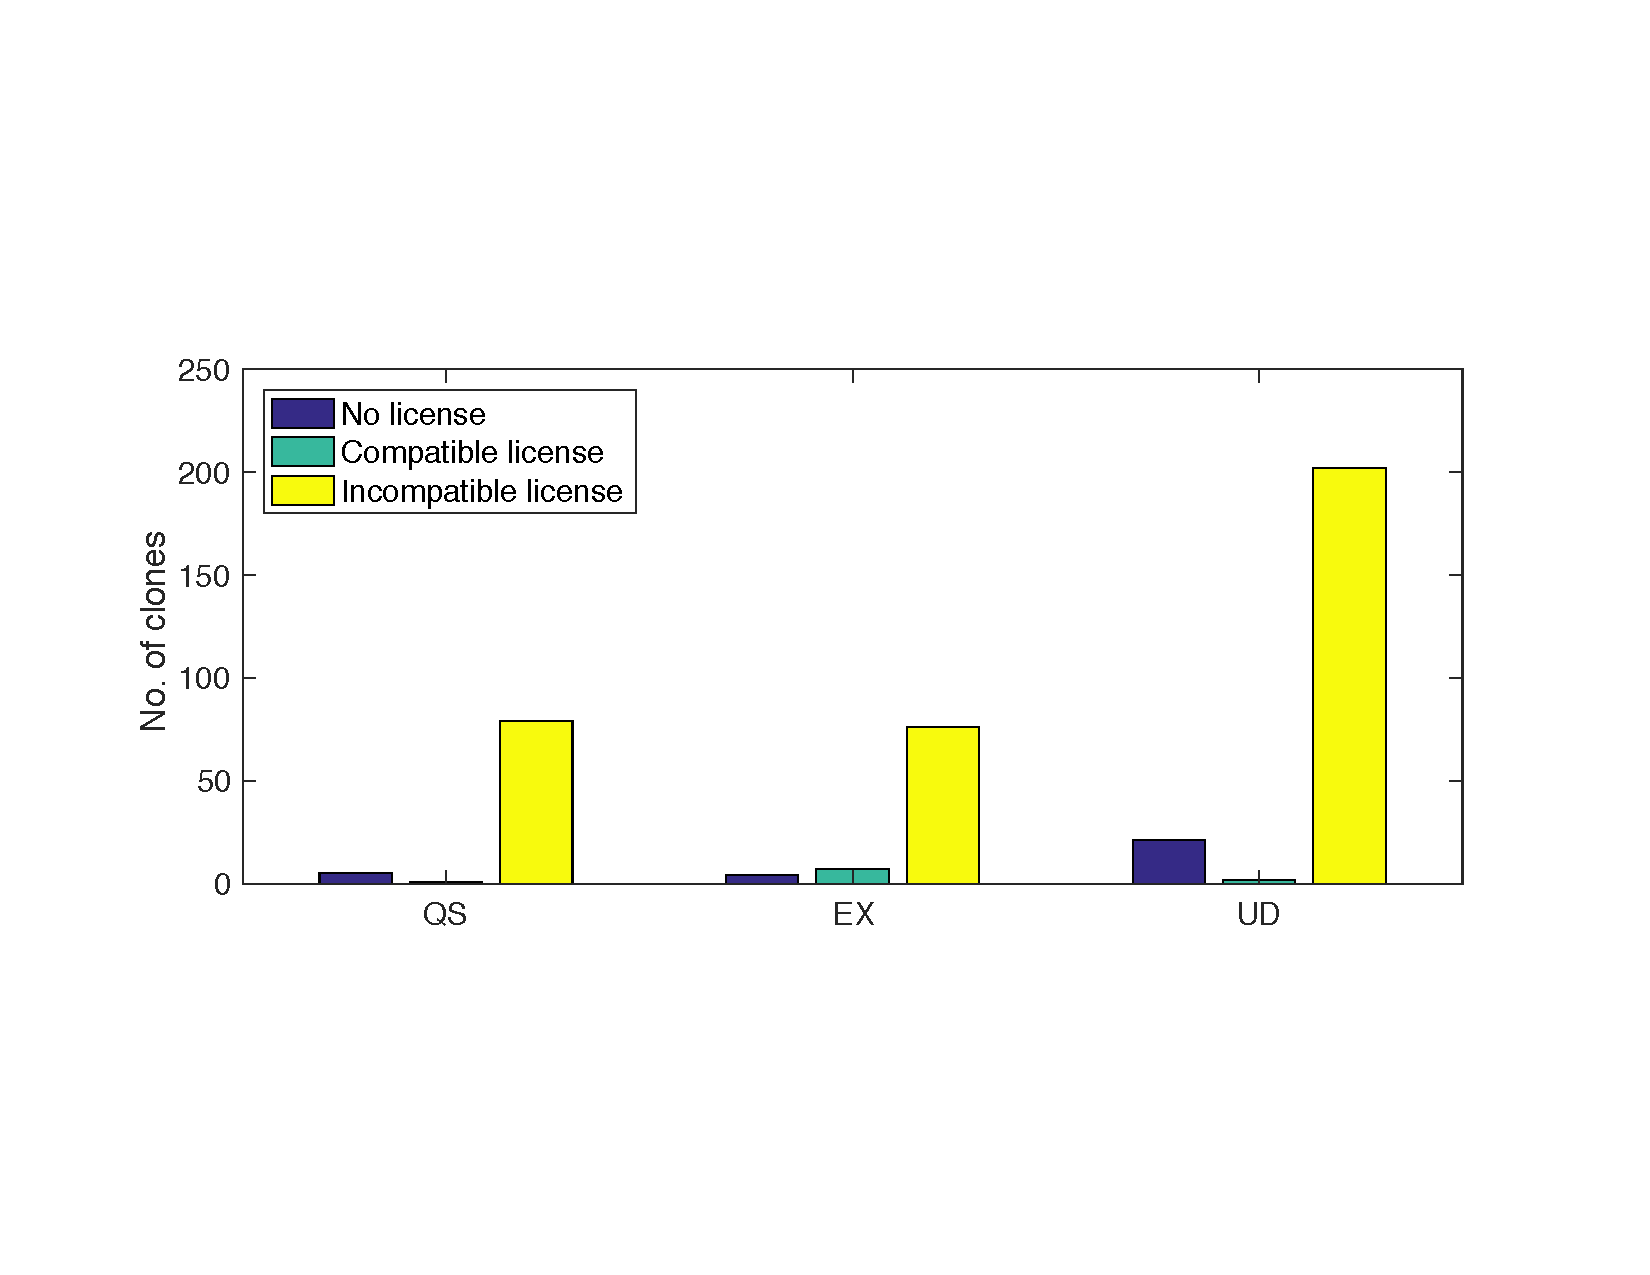
\includegraphics[width=\linewidth]{license_violation}
	\caption{Summary of licensing conflicts in online code clones}
	\label{fig:license_violation}
\end{figure}

\begin{figure*}
		\centering
		\begin{minipage}{.4\textwidth}
			\centering
			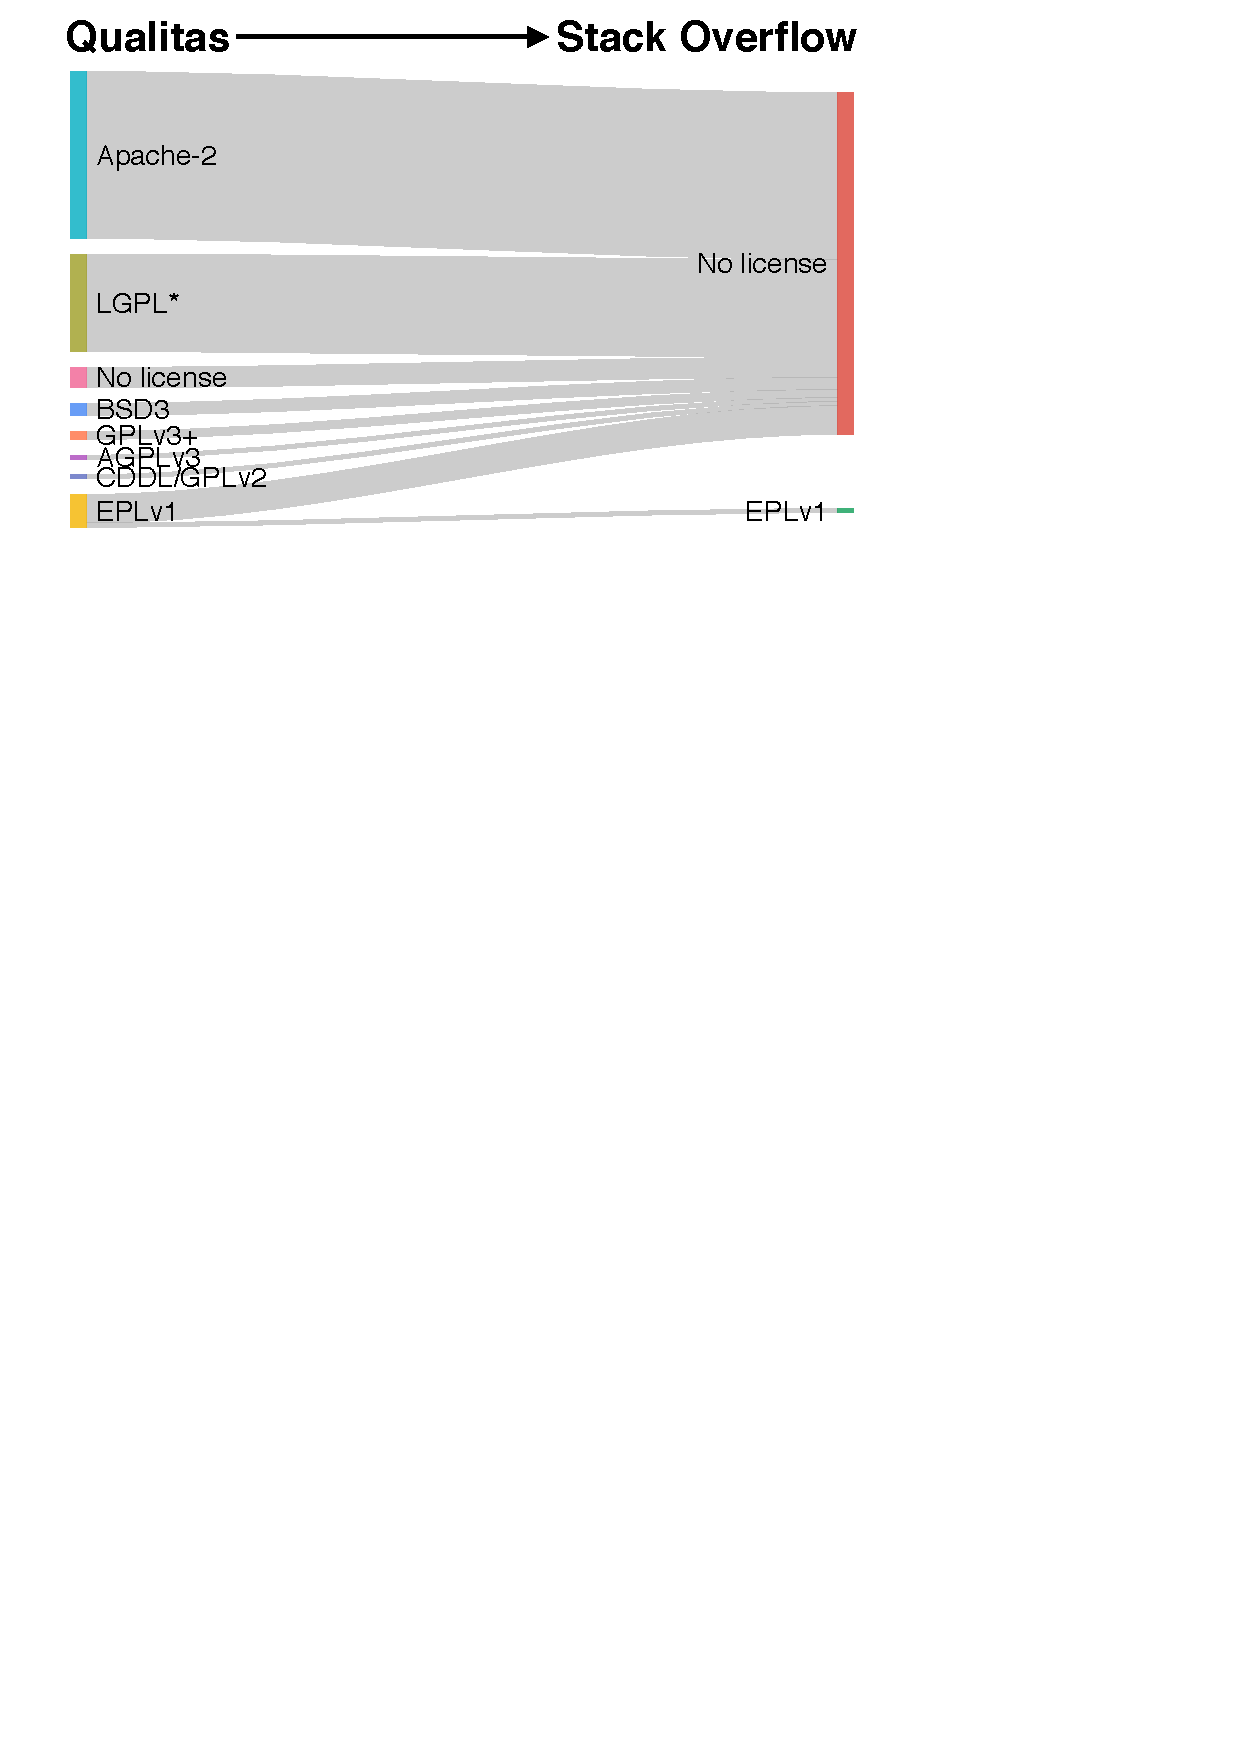
\includegraphics[width=\linewidth]{sankey_license_qs}
			\caption*{(A) QS clones}
		\end{minipage}%
		\hspace{5ex}
		\begin{minipage}{0.4\textwidth}
			\centering
			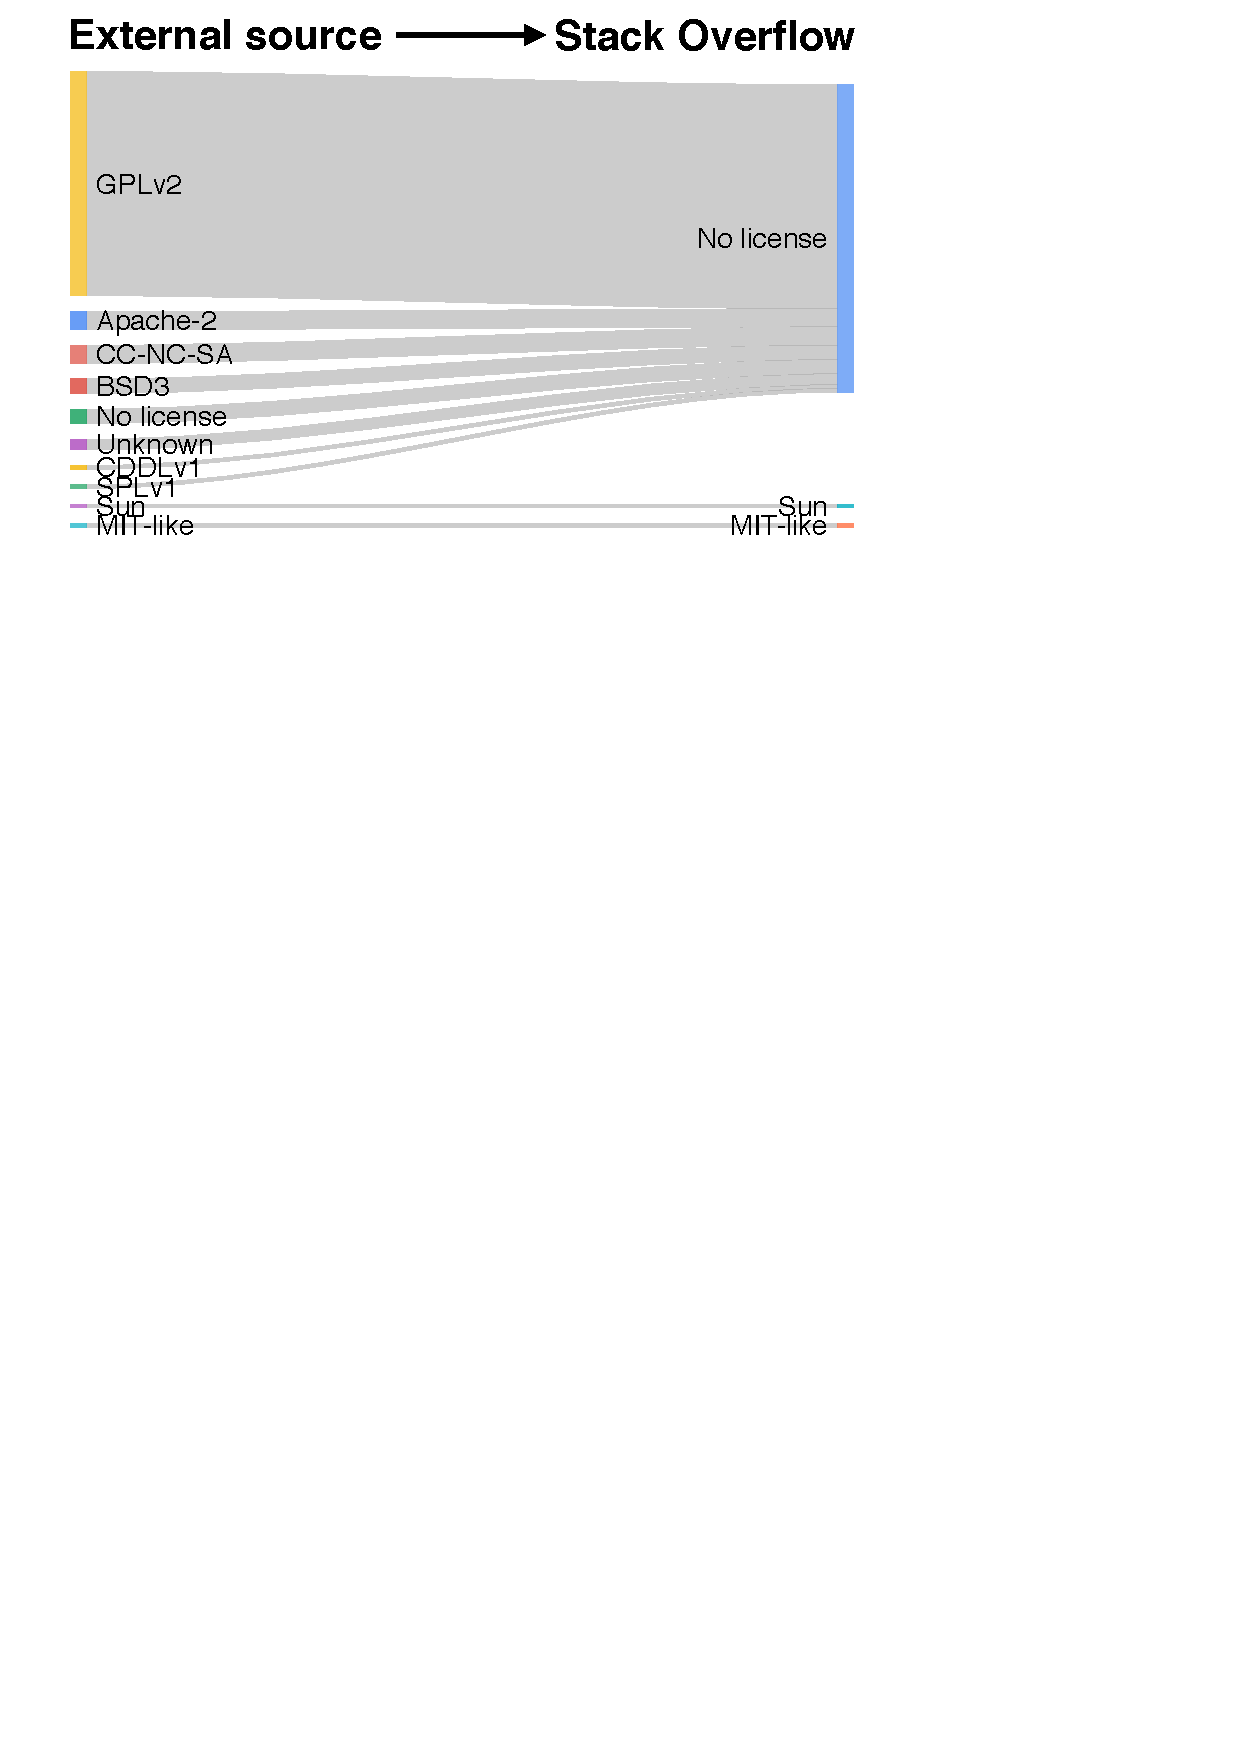
\includegraphics[width=\linewidth]{sankey_license_ex}
			\caption*{(B) EX clones}
		\end{minipage}
	\caption{Direction of changes in online code clone license}
	\label{fig:sankey_license}
\end{figure*}

In our study, we reveal another possible situation of software licensing issues caused by code cloning ``to Stack Overflow''. We found with evidence that 112 pieces of code had been copied from Qualitas projects to Stack Overflow as examples. They are also marked as accepted answers which increased their chances of being reused. The projects came with their respective software licenses (shown in \Cref{t:q_projects_license}). However, we found that the licensing information were mostly stripped from these clones after they were posted on Stack Overflow. The licensing terms on the top of source code are not copied because mostly a small part of the file was cloned to Stack Overflow. If developers copy and reuse these licensed pieces of code in their projects, conflicts may happen without their realisation. 

We analysed licensing conflicts of online clones in QS, UD, and EX set. The summary of licensing information is listed in \Cref{tab:license_abc}. The licenses were extracted by \textbf{Ninka}, an automatic license identification tool~\cite{German2010}. Since Ninka worked at file level, we report the findings based on Stack Overflow snippets and Qualitas source files instead of clone pairs (duplicates were ignored). For the ones that could not be automatically identified by Ninka and had been reported as {\small\texttt{SeeFile}} and {\small\texttt{Unknown}}, we looked at them manually and updated if any license was found.  The table shows license of Stack Overflow snippets and Qualitas source code. The results were reported in groups of QS, UD, and EX. Overall we can see that most of the Stack Overflow snippets do not contain licensing terms while their clone counterparts in Qualitas project do. 

\textbf{No license or compatible license:} There are 31 clone pairs which do not have license on both sides and 8 pairs which have compatible licenses such as Apache license v.2; Eclipse Public License v.1 (EPLv1); No license vs.~Creative Common Attribution-NonCommercial-ShareAlike 3.0 Unported (CC BY-NC-SA 3.0). They are safe for being reused. Since source code and text on Stack Overflow posted before 1st March 2016 are protected by CC BY-NC-SA 3.0 (and MIT license from 1st March 2016 onwards), we can treat Stack Overflow code snippets without licensing information as having CC BY-NC-SA 3.0 by default. CC BY-NC-SA 3.0 license is relaxed and it only request attribution when reuse. 

\textbf{Incompatible license:} there are 359 clone pairs which do not contain licensing information after they are posted on Stack Overflow or having different license from their Qualitas clone counterparts. More than half (79) of QS clone pairs have their licensing terms removed or changed after posted on Stack Overflow. Of 226 UD clone pairs, 202 pairs have incompatible licenses. Again, most of the clones in Qualitas contain license while the Stack Overflow snippets do not. For EX clone pairs, we searched for licensing terms of the original source code from the external sources. We found that 76 out of 87 EX clone pairs have incompatible license. %They are clones that have been identified to be copied from an external source. 
Similarly, their license were removed from Stack Overflow snippets. 

\Cref{fig:sankey_license} shows the direction of changes in online code clone license. The direction of the change is from left to right. The thickness of the line reflects the number of clones for that relationship. In \Cref{fig:sankey_license} (A), we can clearly see that most of the QS online clones have their licenses changed from having a license to ``No license'' on Stack Overflow. The same findings were found for EX online clones as depicted in \Cref{fig:sankey_license} (B). We found that most of the EX clones have their licensing information stripped of after copying to Stack Overflow. These clones are instead covered the default CC BY-NC-SA 3.0 license of Stack Overflow which is strongly permissive. These used-to-be-licensed code are dangerous for being reused because they can implicitly conflicting with the reusing software's license.

\textbf{For RQ4, we found 359 code snippets on Stack Overflow that violate the license of their original software. Majority of them do not contain licensing statements after copied to Stack Overflow.}

\section{Threats to Validity}

\textbf{Internal validity:} 
We could not verify all the 315,786,118 clone pairs reported by the clone detection tools in this study.
Nevertheless, we applied several mechanism to ensure the validity to the subset of clone pairs we classified.
First, we used the two widely-used clone detection tools, Simian and NiCad. We had tried three other clone detectors but could not add them to the study
due to their scalability issue and susceptibility to incomplete code snippets.
Second, we adopted Bellon's clone agreement metric~\cite{Bellon2007} to prioritise and filters clone pairs 
for the manual classification. The agreed clone pairs that passed \textit{good} and \textit{ok} criteria had a higher chance
to be true positive. We also applied the Bellon's clone agreement to 4 different combinations of the tools' configurations.
For disagreed clone pairs, we applied several filters to remove spurious and uninteresting clones. 

The number of online clones we found are subject to the clone detectors and their configurations. 
We mitigated the problem of clone detector's parameter sensitivity by adding another configuration, besides the default one. We reused the established configurations from the EvaClone study~\cite{Wang2013}.
We also performed pairwise matching between the default and EvaClone configurations of the two clone detection tools.

Our seven patterns of online code cloning may not cover all possible online cloning patterns. However, instead of 
defining the patterns beforehand, we resorted to extract them for the data sets. We derived them
from a manual investigation of 679 online clone pairs and adopted one pattern from the study by Kapser et al.~\cite{Kapser2003}.

The 3,632 clone pairs classified manually by the first author are subject to manual judgement and human errors. 
Although we had tried our best to be careful on searching for evidence and classifying the clones, some errors
may still exist. We mitigated this problem by having the second author to validate the classifications with random samplings.
The 64 classification conflicts were discussed and resolved. 
The third author made a final judgement when no consensus could be found by the two authors.
 %In addition, we are aware of voting mechanism
%in Stack Overflow and plan to incorporate highest-vote answers in the future work.

\textbf{External validity:} We carefully chose the data sets for our
experiment so the findings could be generalise as much as possible. 
We selected Stack Overflow because it is one of the most popular programming Q\&A websites available with approximately 6.3 million users.
There are a large number of code snippets reused from the site~\cite{An2017} and there are also several studies encouraging of doing so~(e.g.~\cite{Ponzanelli2013,Ponzanelli2014,Keivanloo2014,Park2014}). 
Nonetheless, it may not be representative to all the programming Q\&A websites. 

Regarding the code snippets, we downloaded the full data dump and extracted Java accepted answers. 
Instead of analysing every post, we only focused on posts marked as accepted answers 
since they are the most likely to being reused. This yields totally 144,075 snippets.
Our findings are limited to these restrictions. They may not be generalised to all programming languages and all
answers on Stack Overflow.

On the other hand, we chose the curated Qualitas corpus for Java open source projects containing 111 projects \cite{QualitasCorpus}.
The projects span over several areas of software and has been used in several empirical studies~\cite{Taube-Schock2011,Beckman2011,Vasilescu2011,Omar2012}. Although it is a curated and well-established corpus, 
it may not fully represent all Java open source software available. 

Lastly, two clone detection tools, Simian and NiCad, are chosen for this study 
due to certain limitations of a few other tools. We have not tried all the tools available 
and they might not be complete representatives of all available clone detection tools.

\section{Related Work}

\textbf{Stack Overflow} is a gold mine for software engineering research. Its rich and developer-driven data are invaluable. Since posts on Stack Overflow may contain code snippets embedded within natural language text, they become a huge database for source code and code-relevant information. The Stack Overflow data set has been put to use in several previous studies. In terms of developer-assisting tools, Seahawk is an Eclipse plug-in that searches and recommends relevant code snippets from Stack Overflow~\cite{Ponzanelli2013}. A follow up work, Prompter, by Ponzanelli et al.~\cite{Ponzanelli2014} achieves the same goal but with improved algorithms. The code snippets on Stack Overflow are mostly examples or solutions to programming problems. Hence, several code search systems use whole or partial data from Stack Overflow as their code search databases~\cite{Keivanloo2014,Park2014, Stolee2014,Subramanian2013,Diamantopoulos2015}. Furthermore, Treude et al.~use machine learning techniques to extract insight sentences from Stack Overflow and use them to improve API documentation~\cite{Treude2016}.

Another aspect is knowledge extraction from Stack Overflow. Nasehi et al.~studied what makes a good code example by analysing answers from Stack Overflow~\cite{Nasehi2012}. Similarly, Yang et al.~\cite{Yang2016} analysed Stack Overflow snippets across various programming languages and observed that code snippets in Python and Javascript are the most usable. Wang et al.~\cite{Wang2013_StackOverflow} use Latent Dirichlet Allocation (LDA) topic modelling to analyse questions and answers from Stack Overflow so that they can automatically categorise new questions. There are also studies trying to understand developers' behaviours on Stack Overflow, e.g.~\cite{Movshovitz-Attias2013,Rosen2016,Choetkiertikul2015,Bosu2013}, while some studies aim to improve Stack Overflow itself~\cite{Diamantopoulos2015, Wang2014}. 

\textbf{Code clone detection} is a long-standing research topic in software engineering. Whether clones are good or bad for software is still controversial~\cite{Sajnani2016,Kapser2003,Kapser2008,Krinke2008,Hotta2010,Gode2011,Harder2013}. However, by only knowing how many code clones residing in software and how they evolve~\cite{Pate2013,Mondal2011} can provide several valuable insights into the software systems. Besides clones, clone detection has its several applications such as software plagiarism detection~\cite{Prechelt2002}, 
source code provenance~\cite{Davies2013}, and software licensing conflicts~\cite{German2009}.

Two code fragments are clones if they are similar enough according to a given definition of similarity~\cite{Bellon2007}. Given an open interpretation of ``definition of similarity'', there are various clone detection tools and their siblings, code plagiarism detectors, invented based on plethora of different code similarity measurements~\cite{Roy2008, Ragkhitwetsagul2016,Svajlenko2014}. Some tools
use string comparison techniques such as Simian~\cite{simian}. NiCad~\cite{Roy2008,Cordy} also exploits Longest Common Subsequence (LCS) string similarity measure to discover clones after applying code pretty-printing using TXL~\cite{Cordy2006}. Many tools do not work on original source code directly but transform them into an
intermediate representation such as tokens and apply similarity
measurement on them. These tools include SourcererCC~\cite{Sajnani2016}, CCFinder~\cite{Kamiya2002},
CP-Miner~\cite{Li2006}, iClones~\cite{Gode2009} and a few more~\cite{Burrows2007, Smith2009, Duric2012, Prechelt2002, Schleimer2003}. 
To find more challenging clones such as clones with added/deleted/reordered statements or equivalent loop and conditional statements (i.e.~type-3 clones), structural similarity of clones is needed.
This structural similarity can be discovered by comparing AST as found in CloneDR~\cite{Baxter1998} and Deckard~\cite{Jiang2007a} or by using program dependence
graphs~\cite{Krinke2001,Komondoor2001}. 

Kapser et al.~studied clones in Linux file systems and create 11 patterns of code cloning based on four groups: Forking, Templating, Customization and Exact match~\cite{Kapser2003,Kapser2008}. Our study partially adapted their patterns for our online code clone classification scheme.

\textbf{Clone agreement} is useful in when clone oracle is absent. Since clone detectors are different in their detection approaches, they may behave differently and report different clones even on the same data set. Some researchers exploit these different behaviours of clone detectors by finding their agreement and obtain highly-confident clones~\cite{Bellon2007,Wang2013}. Using the same data set, clone pairs that are agreed by several tools (or several code similarity measurement techniques) are highly potential to be true clones than the ones reported by only a single tool~\cite{Wang2013,cr2016ssbse,Funaro2010}. These studies also report that sensitivities of the tools' parameter settings have strong effects to the results~\cite{Wang2013,cr2016ssbse}.

\textbf{Software licensing} is crucial for open source and industrial software development. Di Penta et al.~study an evolution of software licensing in six FOSS and found that licensing statements change over time~\cite{DiPenta2010}. German et al.~\cite{German2009} performed an empirical study of code siblings (code clones among different systems coming from the same source) and found that licensing conflicts can occur between the clone siblings. Later, German et al.~\cite{German2010} created Ninka, a tool to automate identification of software license from program source code. We use Ninka to analyse software license from Stack Overflow snippets and Qualitas projects. 

\textbf{Reusing of outdated third-party source code} occurs in software development. Xia et al.~\cite{Xia2014} show that a large number of open source systems reuse outdated third-party libraries from famous open source projects. Using outdated code give detrimental effects to the software since they may introduce vulnerabilities. Our study discovers similar findings in the context of outdated code from Stack Overflow.

The work that is closely similar to us is a study by An et al.~\cite{An2017}. The authors investigated clones between 399 Android apps and Stack Overflow posts. They found 1,226 code snippets which were reused from 68 Android apps. They also observed that there are 1,219 cases of potential license violations. However, the authors rely on the timestamp to judge whether the code has been copied from/to Stack Overflow along with confirmations from six developers. Instead of Android apps, we investigated clones between Stack Overflow and 111 open source projects. Our results confirm their findings that there are clones from software projects to Stack Overflow with potential licensing violations. In our work, we defined seven patterns of online code cloning and performed a large-scale manual check of 3,450 clone pairs. We discovered 96 clone pairs with strong evidences, based on natural text in comments and post contents, that they were copied from Qualitas to Stack Overflow. By comparing the clones to their latest versions in the software, we found that 58 code snippets on Stack Overflow are outdated and harmful for reuse.

\section{Conclusions}
This paragraph will end the body of this sample document.
Remember that you might still have Acknowledgments or
Appendices; brief samples of these
follow.  There is still the Bibliography to deal with; and
we will make a disclaimer about that here: with the exception
of the reference to the \LaTeX\ book, the citations in
this paper are to articles which have nothing to
do with the present subject and are used as
examples only.
%\end{document}  % This is where a 'short' article might terminate

%ACKNOWLEDGMENTS are optional
\section{Acknowledgments}
This section is optional; it is a location for you
to acknowledge grants, funding, editing assistance and
what have you.  In the present case, for example, the
authors would like to thank Gerald Murray of ACM for
his help in codifying this \textit{Author's Guide}
and the \textbf{.cls} and \textbf{.tex} files that it describes.

\begin{figure}
	\centering
	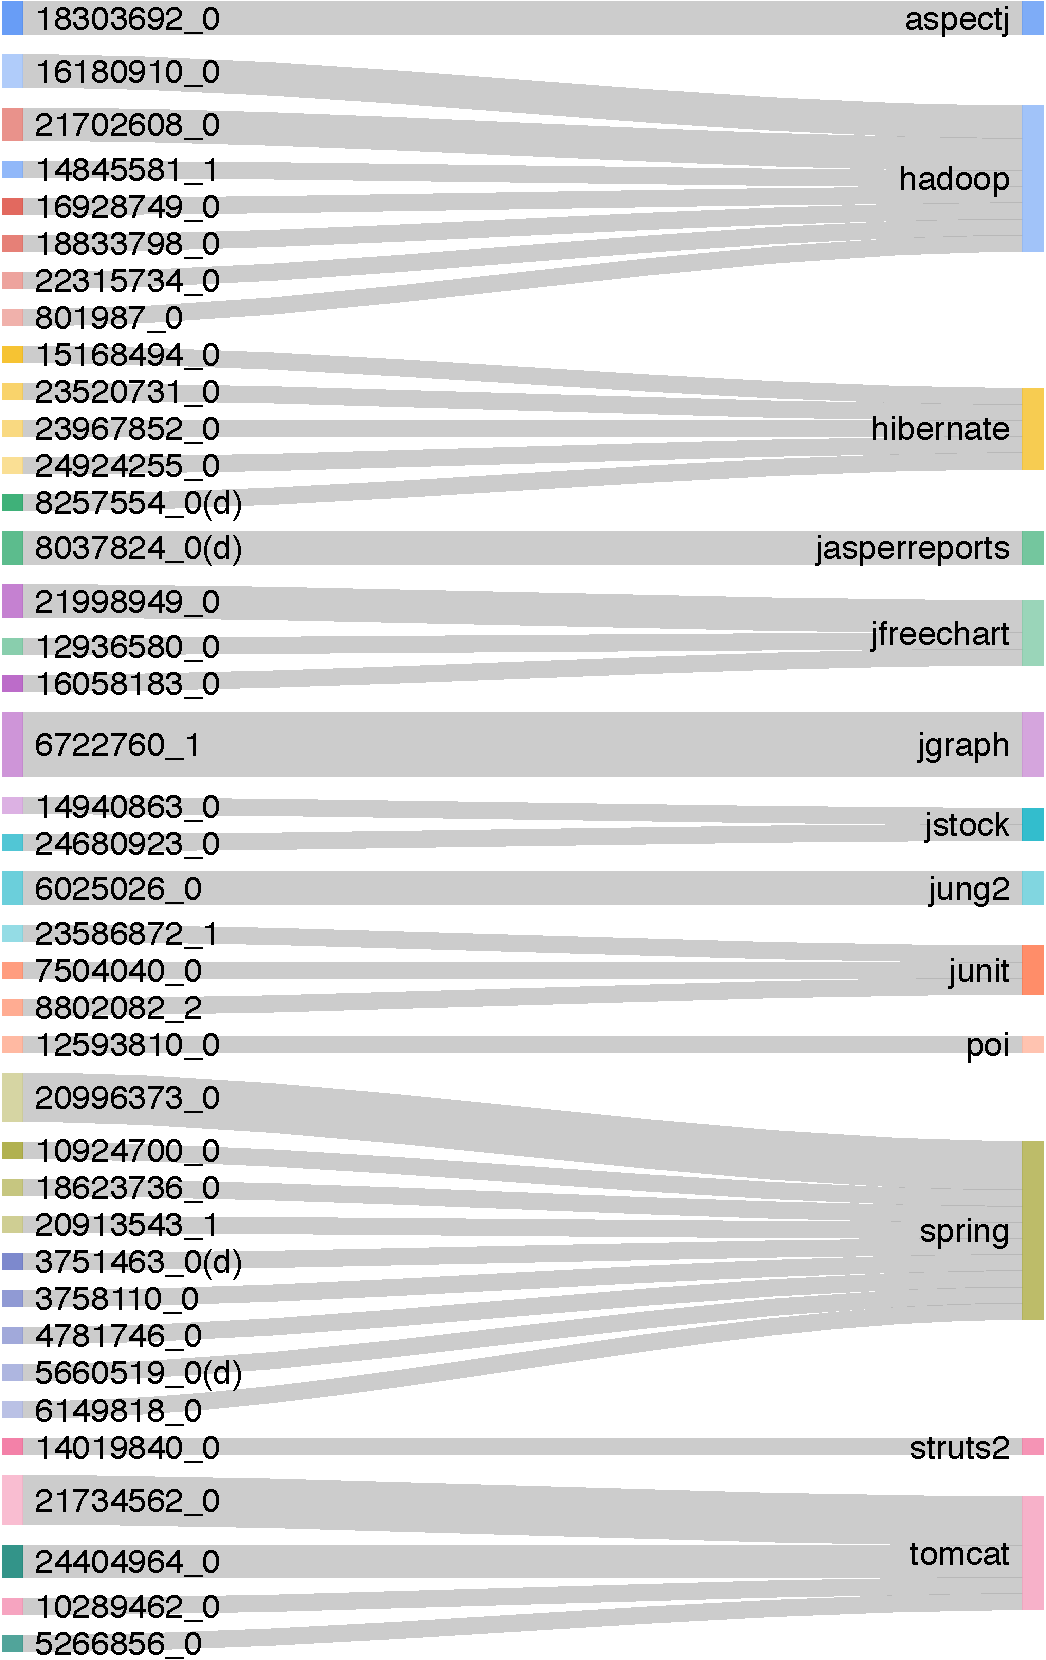
\includegraphics[width=\linewidth]{Sankey_proj}
	\caption{Relationships of 58 Stack Overflow clone pairs to their original projects. 55 are outdated and 3 are deleted (shown using (d) suffix).}
	\label{fig:sankey}
\end{figure}

%
% The following two commands are all you need in the
% initial runs of your .tex file to
% produce the bibliography for the citations in your paper.
\bibliographystyle{abbrv}
\bibliography{sigproc}  

\end{document}
